\documentclass[11 pt]{beamer}

\usepackage[utf8]{inputenc}
\usepackage[T1]{fontenc}
\usepackage[french]{babel}

\usepackage{amsmath}
\usepackage{empheq}
\usepackage{tikz}
\usepackage{tikz-qtree}
\usepackage{listings}
\usepackage{graphicx}
\usepackage{textcomp}

\usepackage{xmpmulti}
\usepackage{animate}

\usetheme{Antibes}

\setbeamertemplate{itemize subitem}[square]
\setbeamertemplate{itemize subsubitem}[circle]
\setbeamertemplate{footline}[frame number]

\title{Classification of points in a euclidean space}
\author{Luc Blassel, Romain Gautron}

\begin{document}
\maketitle

\begin{frame}{Our problem}
	\begin{figure}
		\centering
		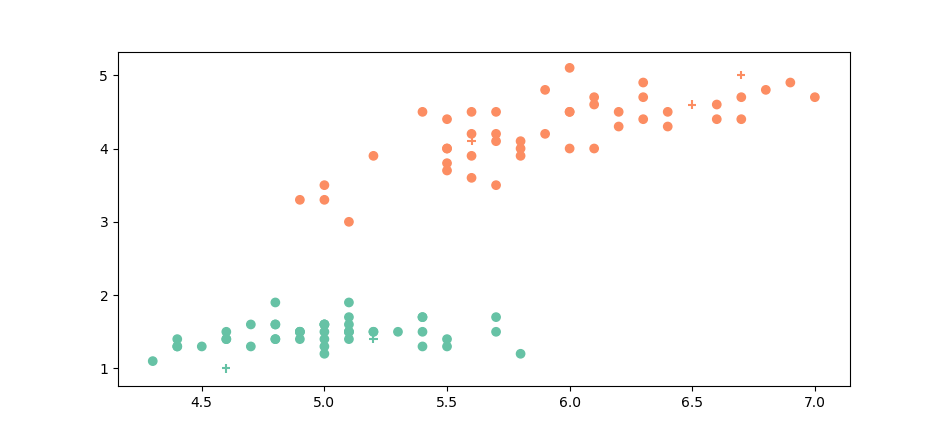
\includegraphics[width=\textwidth]{figures/irisClass.png}
		\caption{Classification problem in euclidean space}
		\label{fig:iris}
	\end{figure}
\end{frame}
%
% %%%%%%%%%%%%%%%%%%%%%%%%%%%%%%%%%%%%%%%%%%%%%%%%%%%%%%%%%%%%%%%%%%%%

\begin{frame}{Our problem}
	Let $S$ be a set of $I$ points of $\mathbf{R^d}$.

	\medskip

	Each element of $S$ has a known label $y_i$ in $\{-1,1\}$.

	\medskip

	Let $U$ be a set of $\mathbf{R^d}$ points  for which we don't know the labels.

	\medskip

	We suppose that $S$ and $U$ come from the same ensemble.

	\medskip

	We want to assign labels from $\{-1,1\}$ to the points of $U$.

\end{frame}
%
% %%%%%%%%%%%%%%%%%%%%%%%%%%%%%%%%%%%%%%%%%%%%%%%%%%%%%%%%%%%%%%%%%%%%

\begin{frame}{Our problem}
A lot of ways to solve it :

\begin{itemize}
	\item generative approach
%
	\textrightarrow learning the distribution of individual classes

		\begin{itemize}
			\item Naives Bayes
			\item Logistic regression
			\item ...
		\end{itemize}
  %
	\item discriminative approach
  %
	\textrightarrow learning the boundaries between classes

		\begin{itemize}
			\item KNN
			\item Random Forest
			\item LDA
			\item NNets
			\item ...
		\end{itemize}
\end{itemize}
\end{frame}
% %%%%%%%%%%%%%%%%%%%%%%%%%%%%%%%%%%%%%%%%%%%%%%%%%%%%%%%%%%%%%%%%%%%%

\section{The KNN problem}

%%%%%%%%%%%%%%%%%%%%%%%%%%%%%%%%%%%%%%%%%%%%%%%%%%%%%%%%%%%%%%%%%%%%

\begin{frame}{Our framework}
Discriminative approach : KNN
\begin{itemize}
	\item simple algorithm
	\item well performing
	\item non linear
\end{itemize}

\Large{\textrightarrow we will deal with the multiclass case}
\end{frame}

%%%%%%%%%%%%%%%%%%%%%%%%%%%%%%%%%%%%%%%%%%%%%%%%%%%%%%%%%%%%%%%%%%%%

\begin{frame}{The KNN algorithm}
\begin{block}{KNN principle (1)}
In order to assign a label to an unknown point :
\begin{enumerate}
	\item find the k-nearest neighbours according to a distance
	\item take the majority of the corresponding labels ; if equality pick one randomly
\end{enumerate}
\end{block}
\end{frame}

%%%%%%%%%%%%%%%%%%%%%%%%%%%%%%%%%%%%%%%%%%%%%%%%%%%%%%%%%%%%%%%%%%%%

\begin{frame}{KNN principle (2)}
\begin{figure}
	\centering
	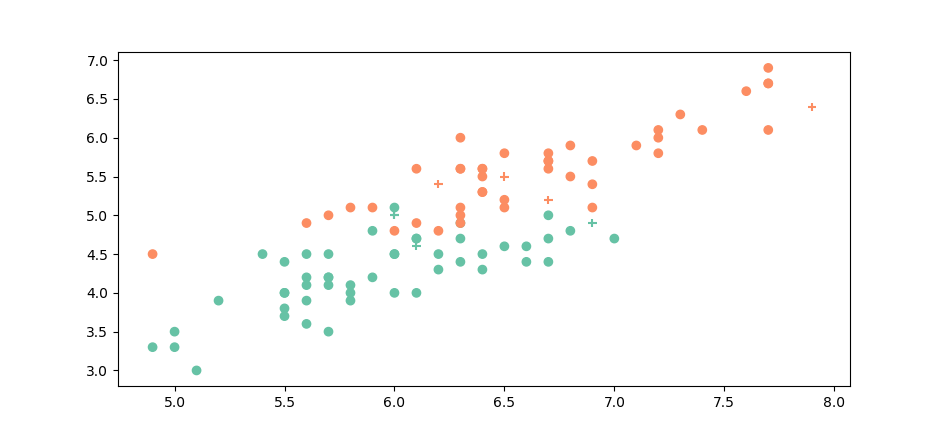
\includegraphics[width=\textwidth]{figures/irisClass2_1.png}
	\caption{KNN example}
	\label{fig:iris2}
\end{figure}
\end{frame}
%
% %%%%%%%%%%%%%%%%%%%%%%%%%%%%%%%%%%%%%%%%%%%%%%%%%%%%%%%%%%%%%%%%%%%%

\begin{frame}{Naive KNN approach}
Given an unknown point $X$ :
\begin{enumerate}
	\item compute all the distances :

	for $s \in S, i \in I :\Vert s_i - X\Vert$

	\item sort the distances and select the k-least

	\item take the majority of the corresponding labels ; if equality pick one randomly
\end{enumerate}

Given a space dimension $d$, research costs for one unknown point (assuming $k \ll n$) :

\begin{itemize}
	\item $o(d)$ per known point
	\item $o(nd)$ for the whole data set
\end{itemize}

Space complexity is $o(dn)$
\end{frame}
%
% %%%%%%%%%%%%%%%%%%%%%%%%%%%%%%%%%%%%%%%%%%%%%%%%%%%%%%%%%%%%%%%%%%%%
\section{KNN improvements}
%%%%%%%%%%%%%%%%%%%%%%%%%%%%%%%%%%%%%%%%%%%%%%%%%%%%%%%%%%%%%%%%%%%%

\begin{frame}{How to improve naive knn ?}
\begin{itemize}
	\item approximate knn
	\item exact knn
\end{itemize}

\textrightarrow based on pre-partionning the space
\end{frame}
%
% %%%%%%%%%%%%%%%%%%%%%%%%%%%%%%%%%%%%%%%%%%%%%%%%%%%%%%%%%%%%%%%%%%%%
% \subsection{Approximate knn}
% %%%%%%%%%%%%%%%%%%%%%%%%%%%%%%%%%%%%%%%%%%%%%%%%%%%%%%%%%%%%%%%%%%%%

\begin{frame}{LSH approach}
Random hyperplan \textrightarrow hash function
\begin{figure}
	\centering
	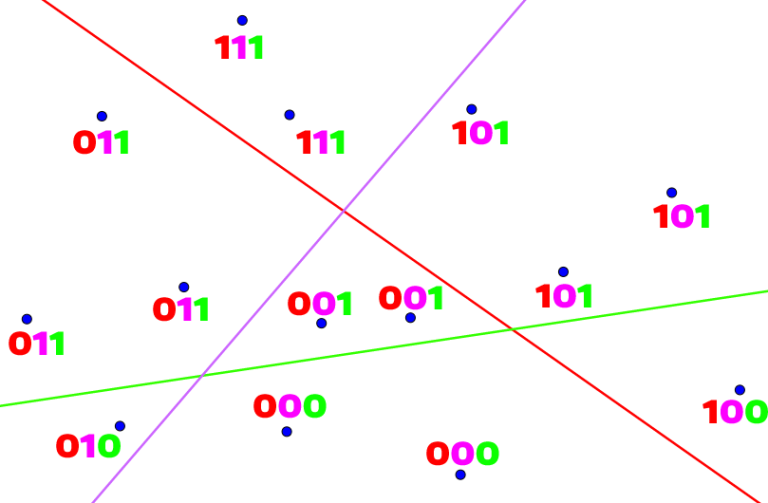
\includegraphics[width=.45\textwidth]{figures/lsh.png}
	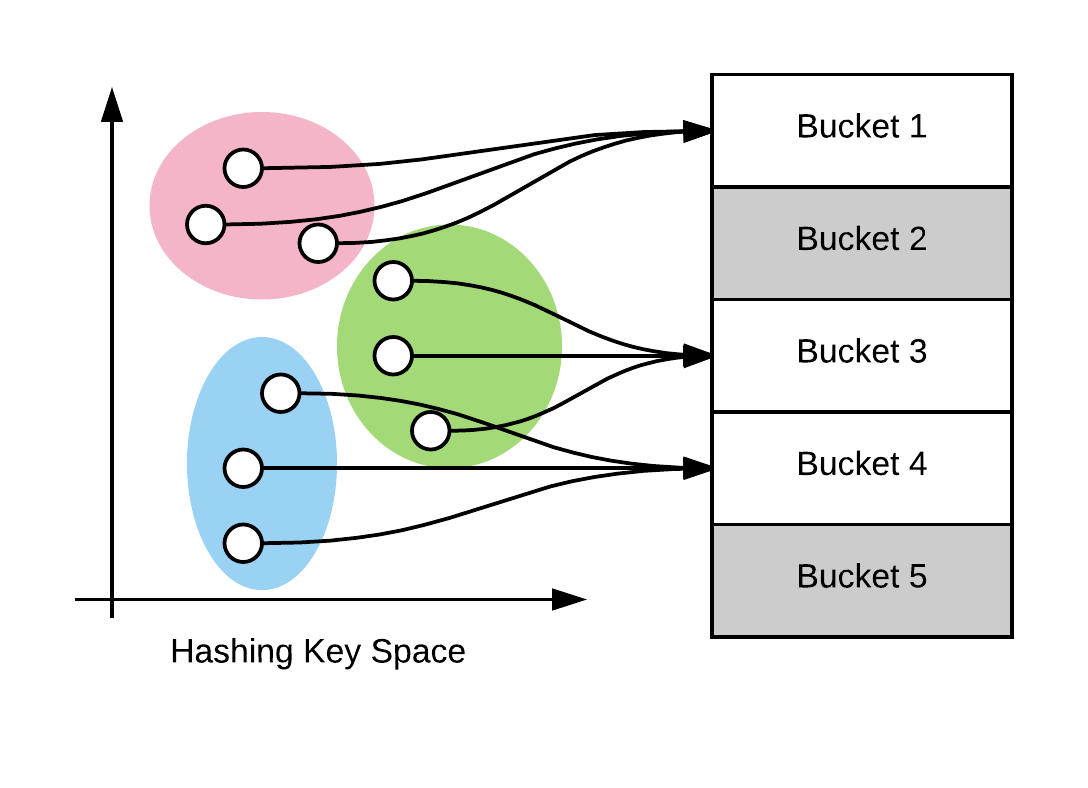
\includegraphics[width=.45\textwidth]{figures/lsh2.png}
	\caption{LSH}
	\label{fig:lsh2}
\end{figure}

The region where falls the new point gives the candidates
\\
Repeat it - gather candidates - compute distances

$o(kd + \frac{nd}{2^k})\approx o(dlog(n))$


\end{frame}
% %%%%%%%%%%%%%%%%%%%%%%%%%%%%%%%%%%%%%%%%%%%%%%%%%%%%%%%%%%%%%%%%%%%%
\subsection{approximate k-NN}

\begin{frame}{KD trees V1}
\begin{figure}
	\centering
	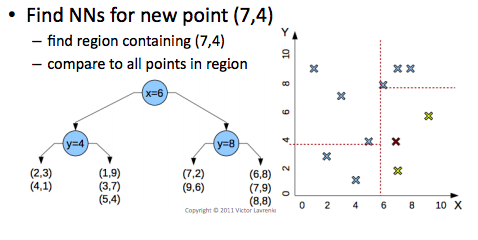
\includegraphics[width=\textwidth]{figures/lavrenko.png}
	\caption{KD trees V1 (copyright V. Lavrenko)}
	\label{fig:lsh}
\end{figure}
$o(log(n)+kd)$
\end{frame}
%
%%%%%%%%%%%%%%%%%%%%%%%%%%%%%%%%%%%%%%%%%%%%%%%%%%%%%%%%%%%%%%%%%%%%
\subsection{Exact knn}
%%%%%%%%%%%%%%%%%%%%%%%%%%%%%%%%%%%%%%%%%%%%%%%%%%%%%%%%%%%%%%%%%%%%

\begin{frame}{KD trees V2}
\Large{\textrightarrow KDtrees with exact NNs : our work !}
\end{frame}

\begin{frame}[c]{A simple example}
  We have the following dataset in a $2d$ space:
  \begin{align*}
    X &=\{(1, 3),(1, 8), (2, 2), (2, 10), (3, 6), (4, 1), (5, 4), (6, 8), \\&(7, 4), (7, 7), (8, 2), (8, 5), (9, 9)\}\\
    &\\
    Y &= \{Blue,\ Blue,\ Blue,\ Blue,\ Blue,\ Blue,\ Red,\ Red,\ Red,\ Red,\ \\& Red,\ Red,\ Red \}
  \end{align*}
  We want to assign a color to the following point: $(4,8)$\
\end{frame}
%
\begin{frame}{How to opitimze k-nn search}
  We use a data structure known as a k-d tree.
\end{frame}
%
\begin{frame}[shrink=22]{building the k-d tree}
  \begin{tikzpicture}[draw,circle,fill=none]
    \node[draw,fill=red] (0) at (0,0) {$(5,4)$};

    \node[draw,fill=green] (1) at (-4,-2) {$(3,6)$};
    \node[draw,fill=green] (2) at (4,-2 ) {$(7,7)$};

    \node[draw,fill=red] (3) at (-6,-4) {$(2,2)$};
    \node[draw,fill=red] (4) at (-2,-4) {$(2,10)$};
    \node[draw,fill=red] (5) at (2,-4 ) {$(8,2)$};
    \node[draw,fill=red] (6) at (6,-4 ) {$(9,9)$};

    \node[draw,fill=green] (7) at (-7,-6) {$(1,3)$};
    \node[draw,fill=green] (8) at (-5,-6) {$(4,1)$};
    \node[draw,fill=green] (9) at (-3,-6) {$(1,8)$};
    \node[draw,fill=green] (10) at (1,-6) {$(7,4)$};
    \node[draw,fill=green] (11) at (3,-6) {$(8,5)$};
    \node[draw,fill=green] (12) at (5,-6) {$(6,8)$};

    \draw (0)--(1);
    \draw (0)--(2);
    \draw (1)--(3);
    \draw (1)--(4);
    \draw (2)--(5);
    \draw (2)--(6);
    \draw (3)--(7);
    \draw (3)--(8);
    \draw (4)--(9);
    \draw (5)--(10);
    \draw (5)--(11);
    \draw (6)--(12);
  \end{tikzpicture}
\end{frame}

\begin{frame}{How do we partition the space?}
  \centering
  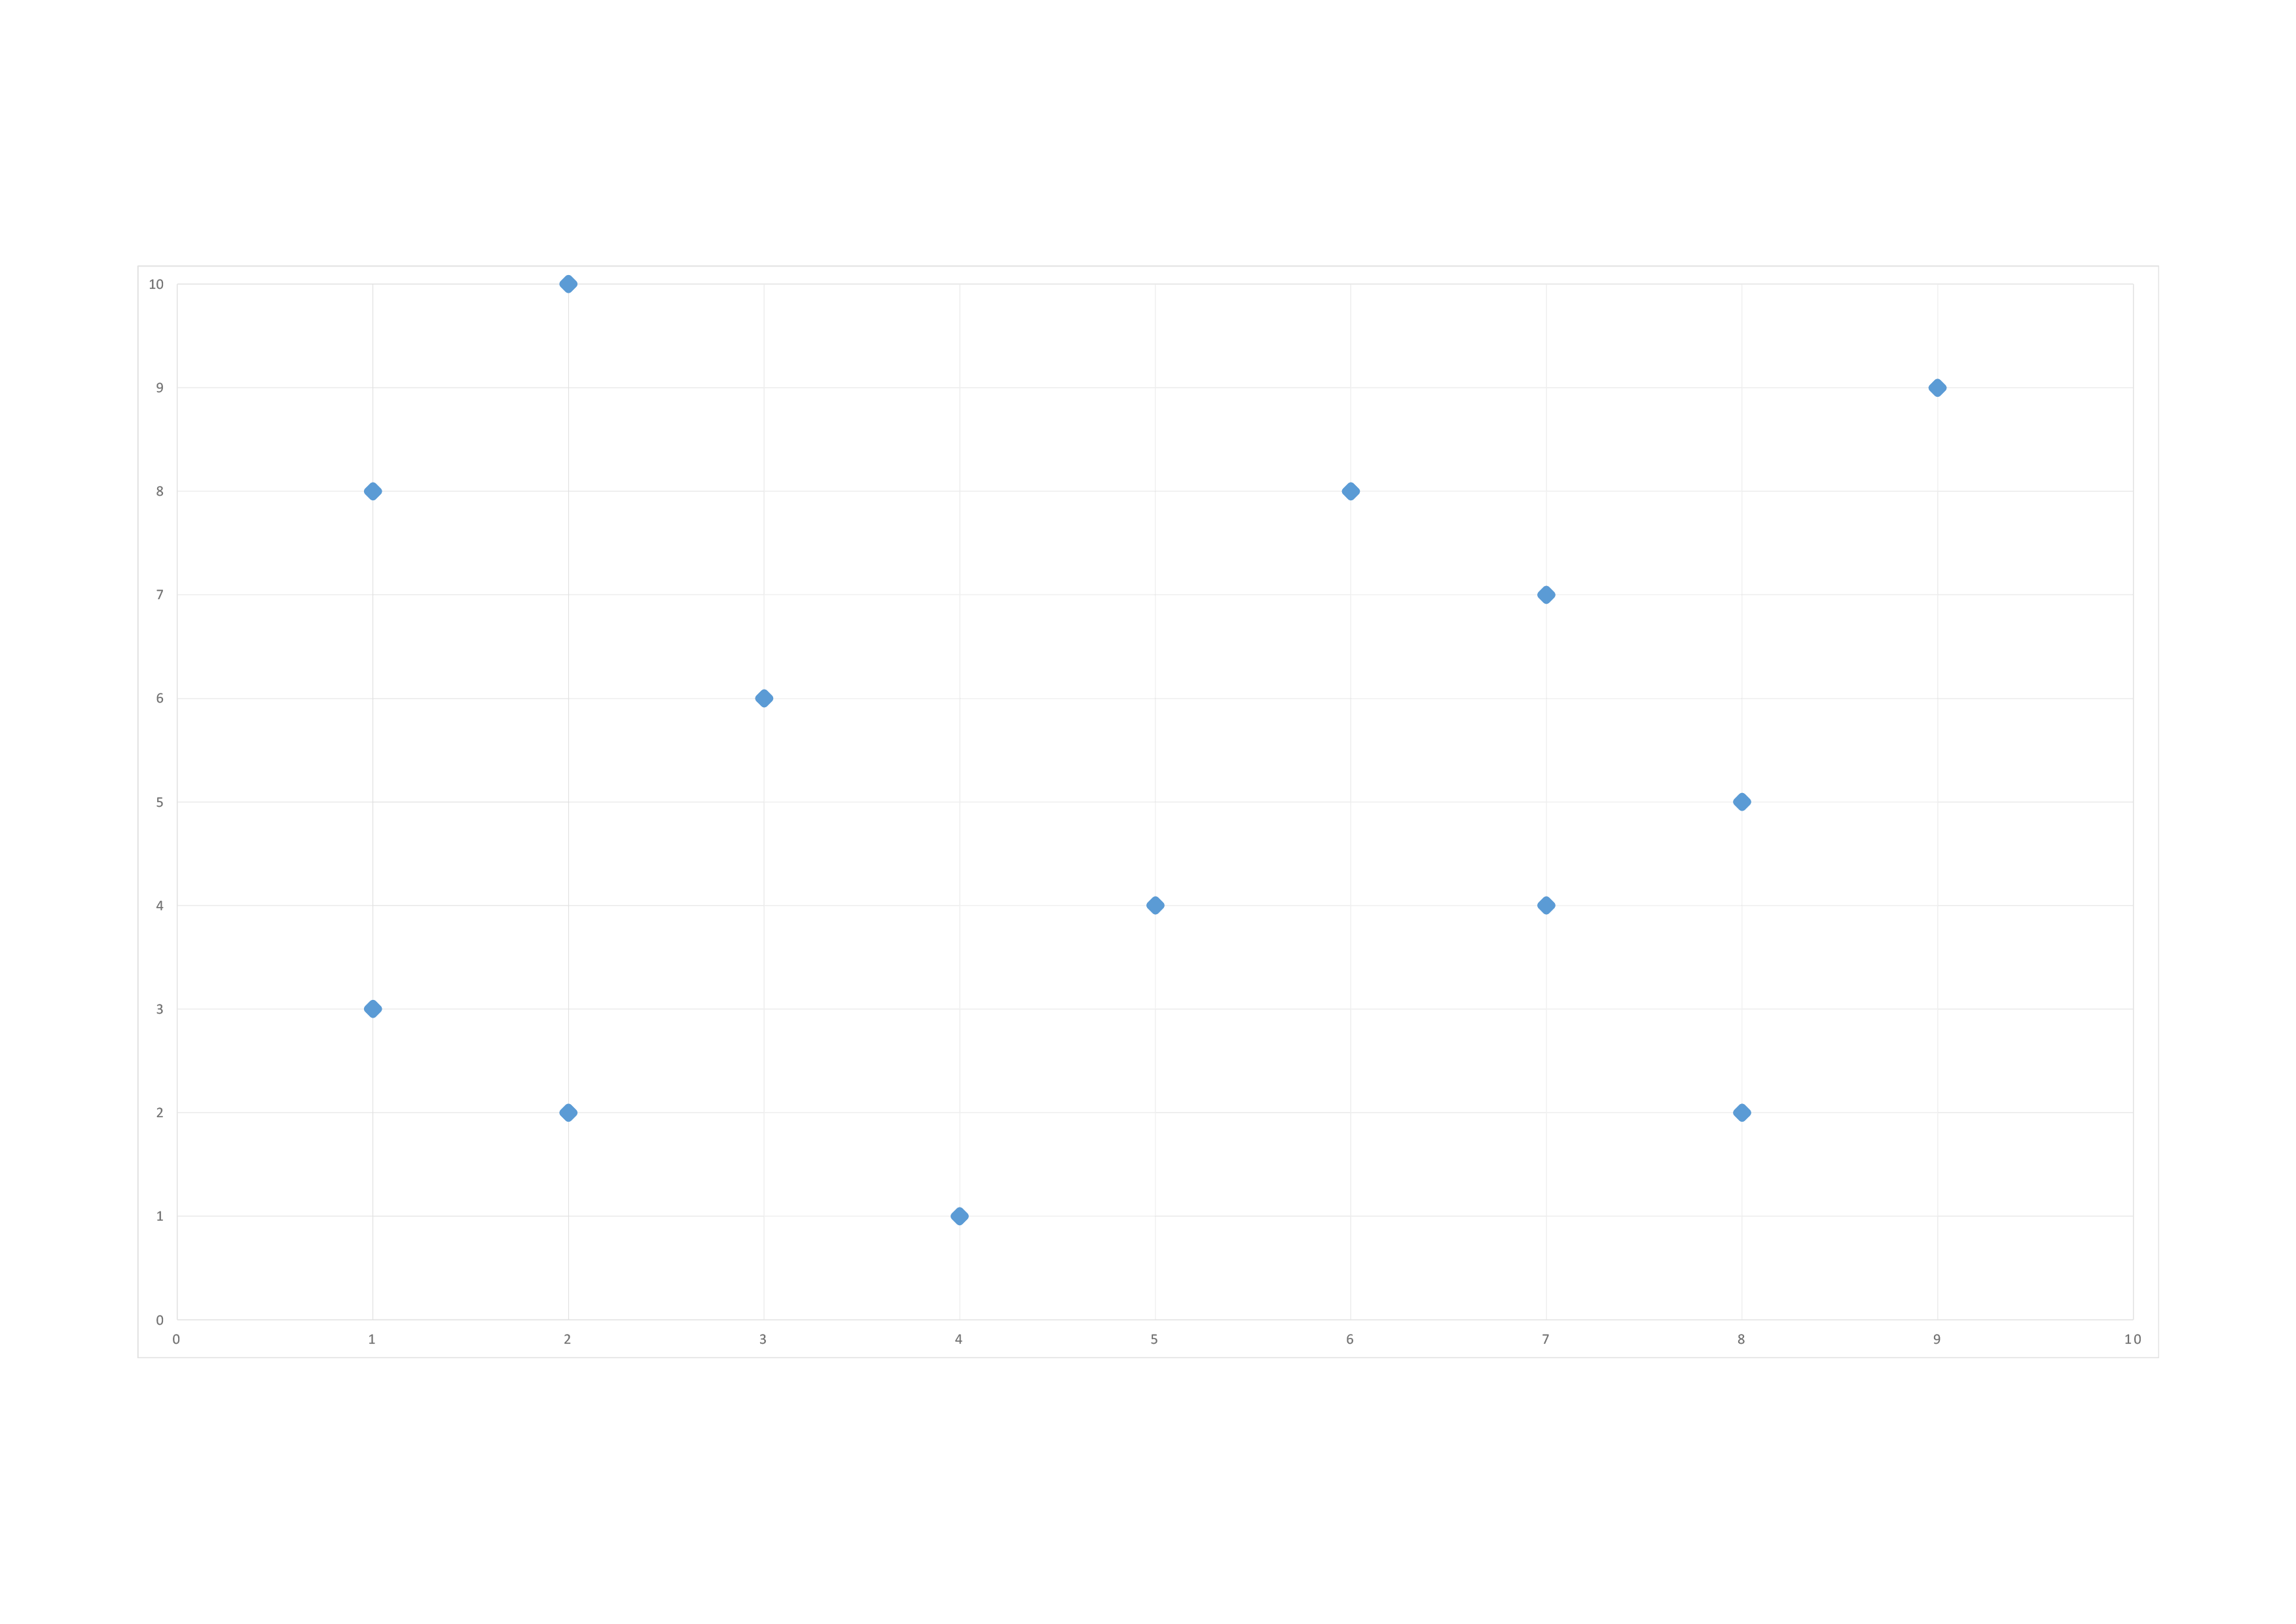
\includegraphics[width=.7\textwidth]{figures/Base.png}
\end{frame}
\begin{frame}{How do we partition the space?}
  \centering4
    \only<1>{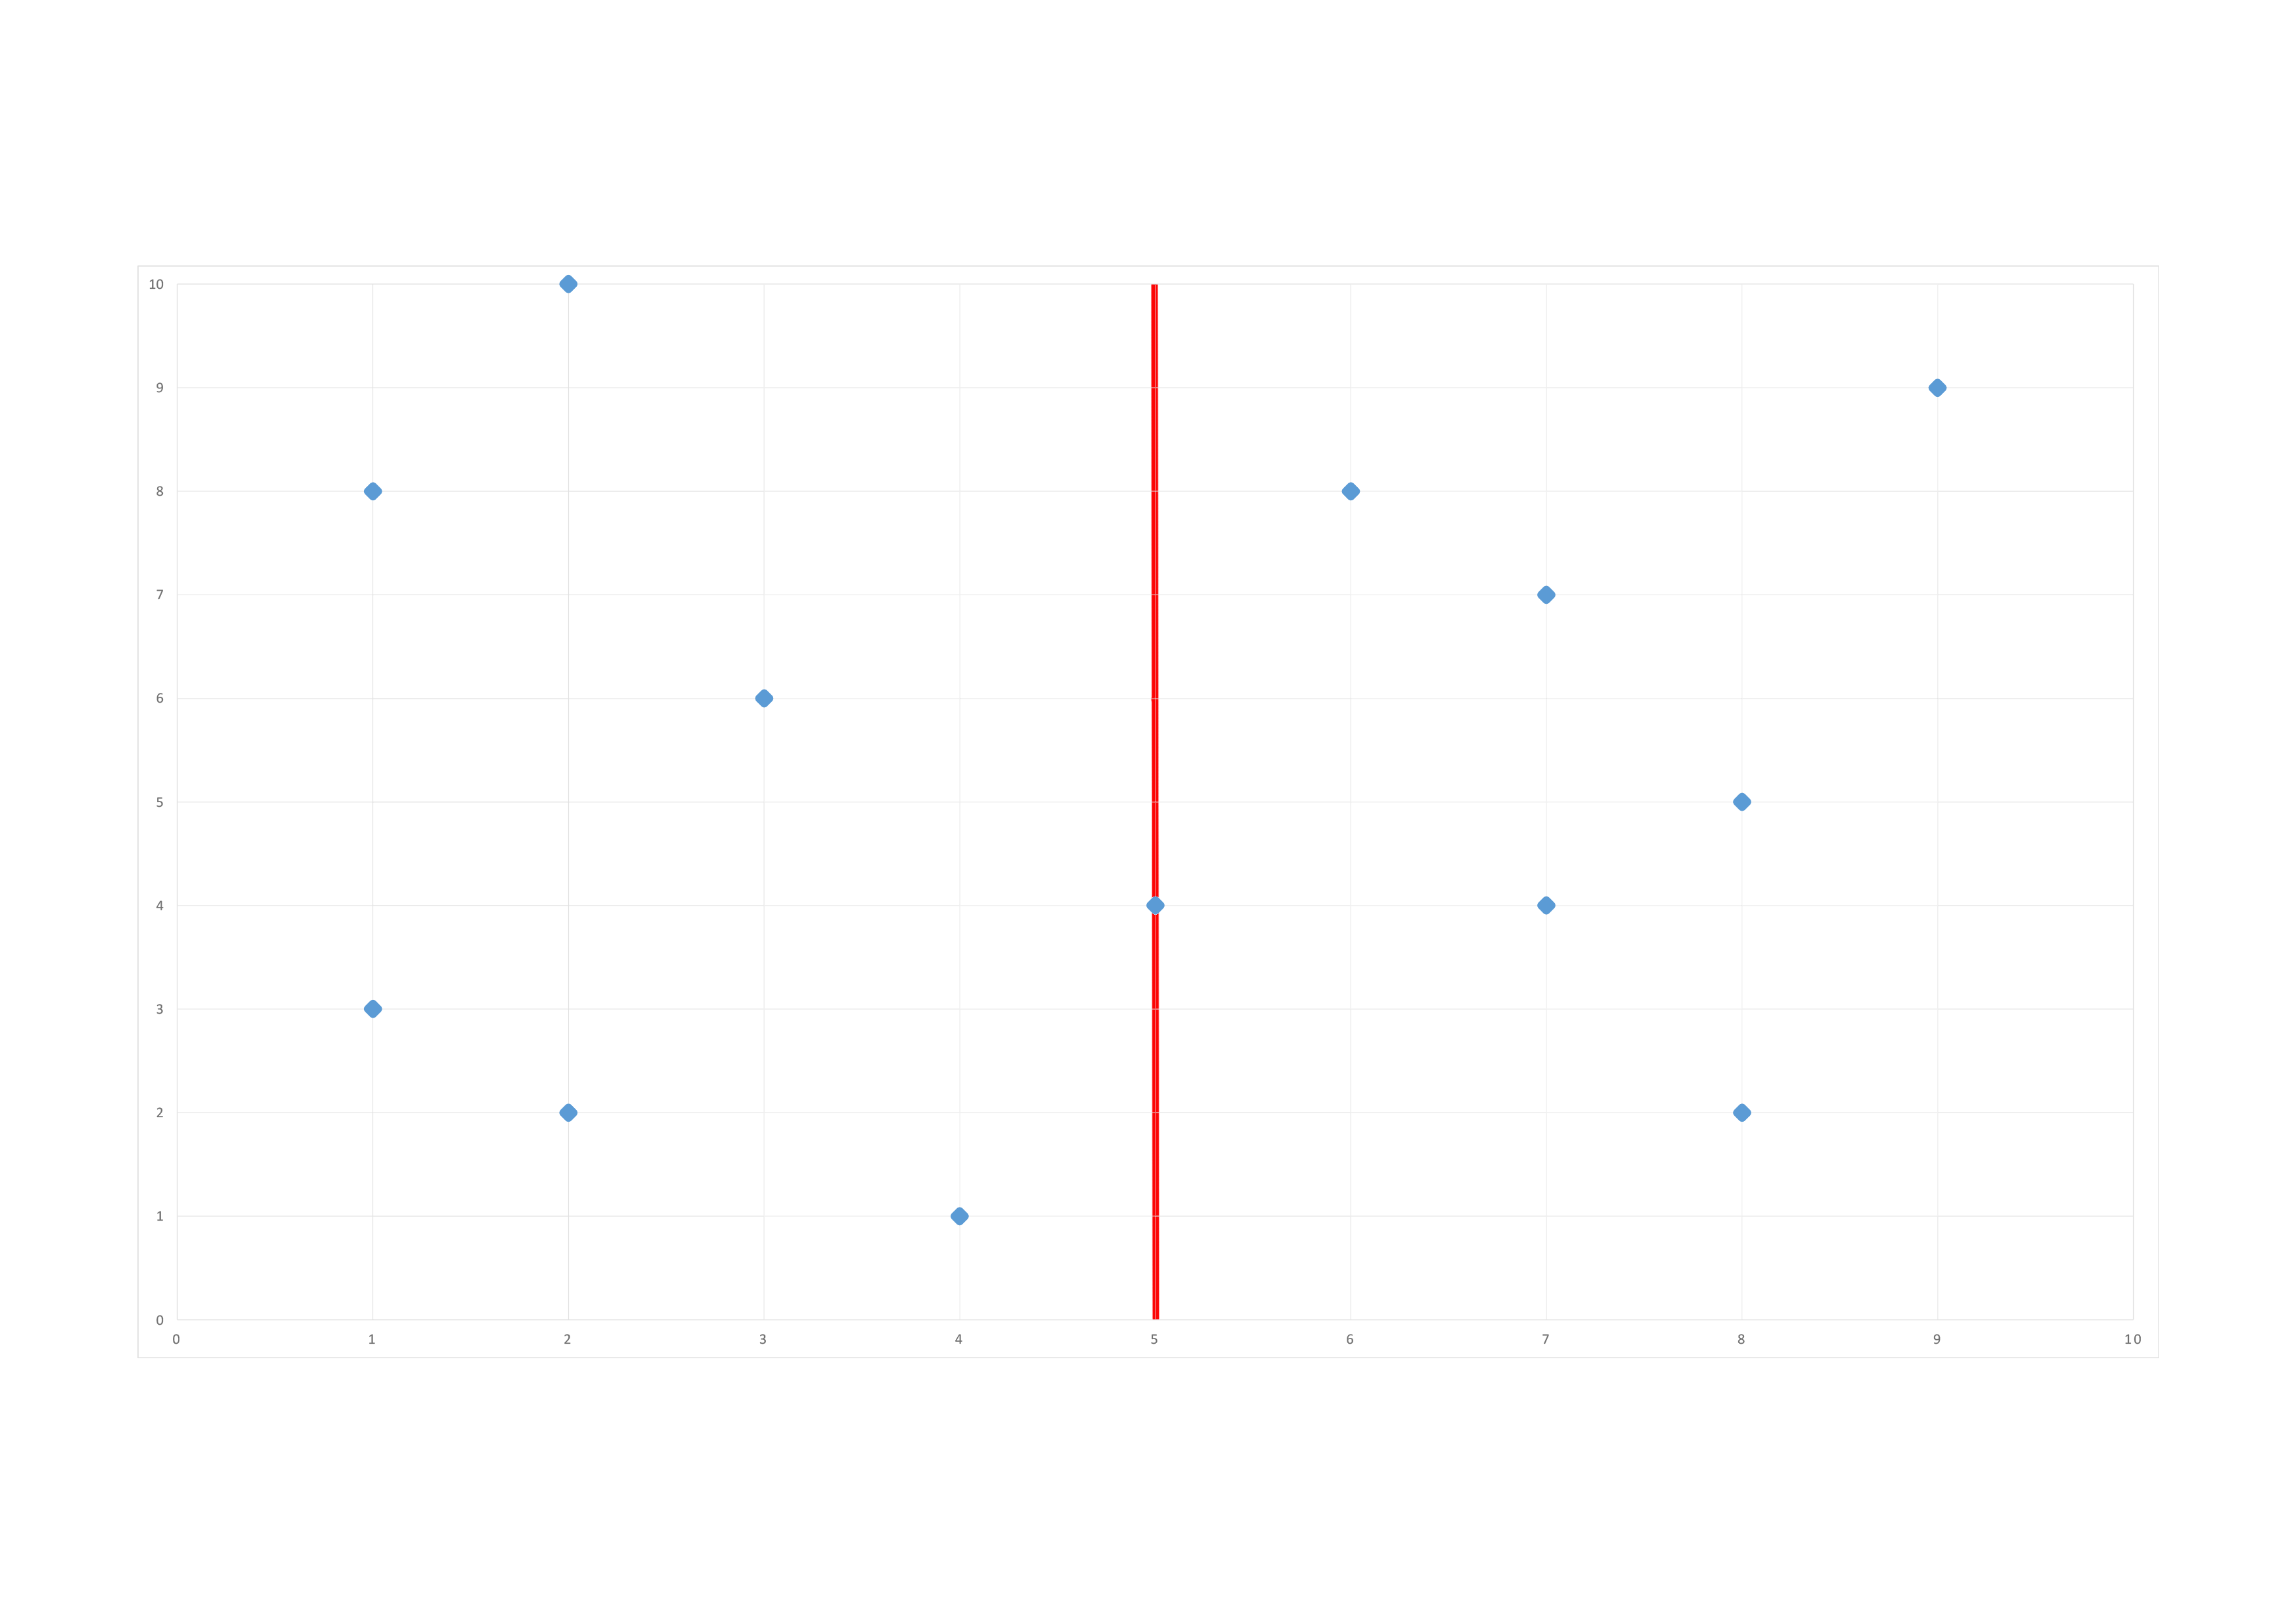
\includegraphics[width=.7\textwidth]{figures/split1.png}}
    \only<2>{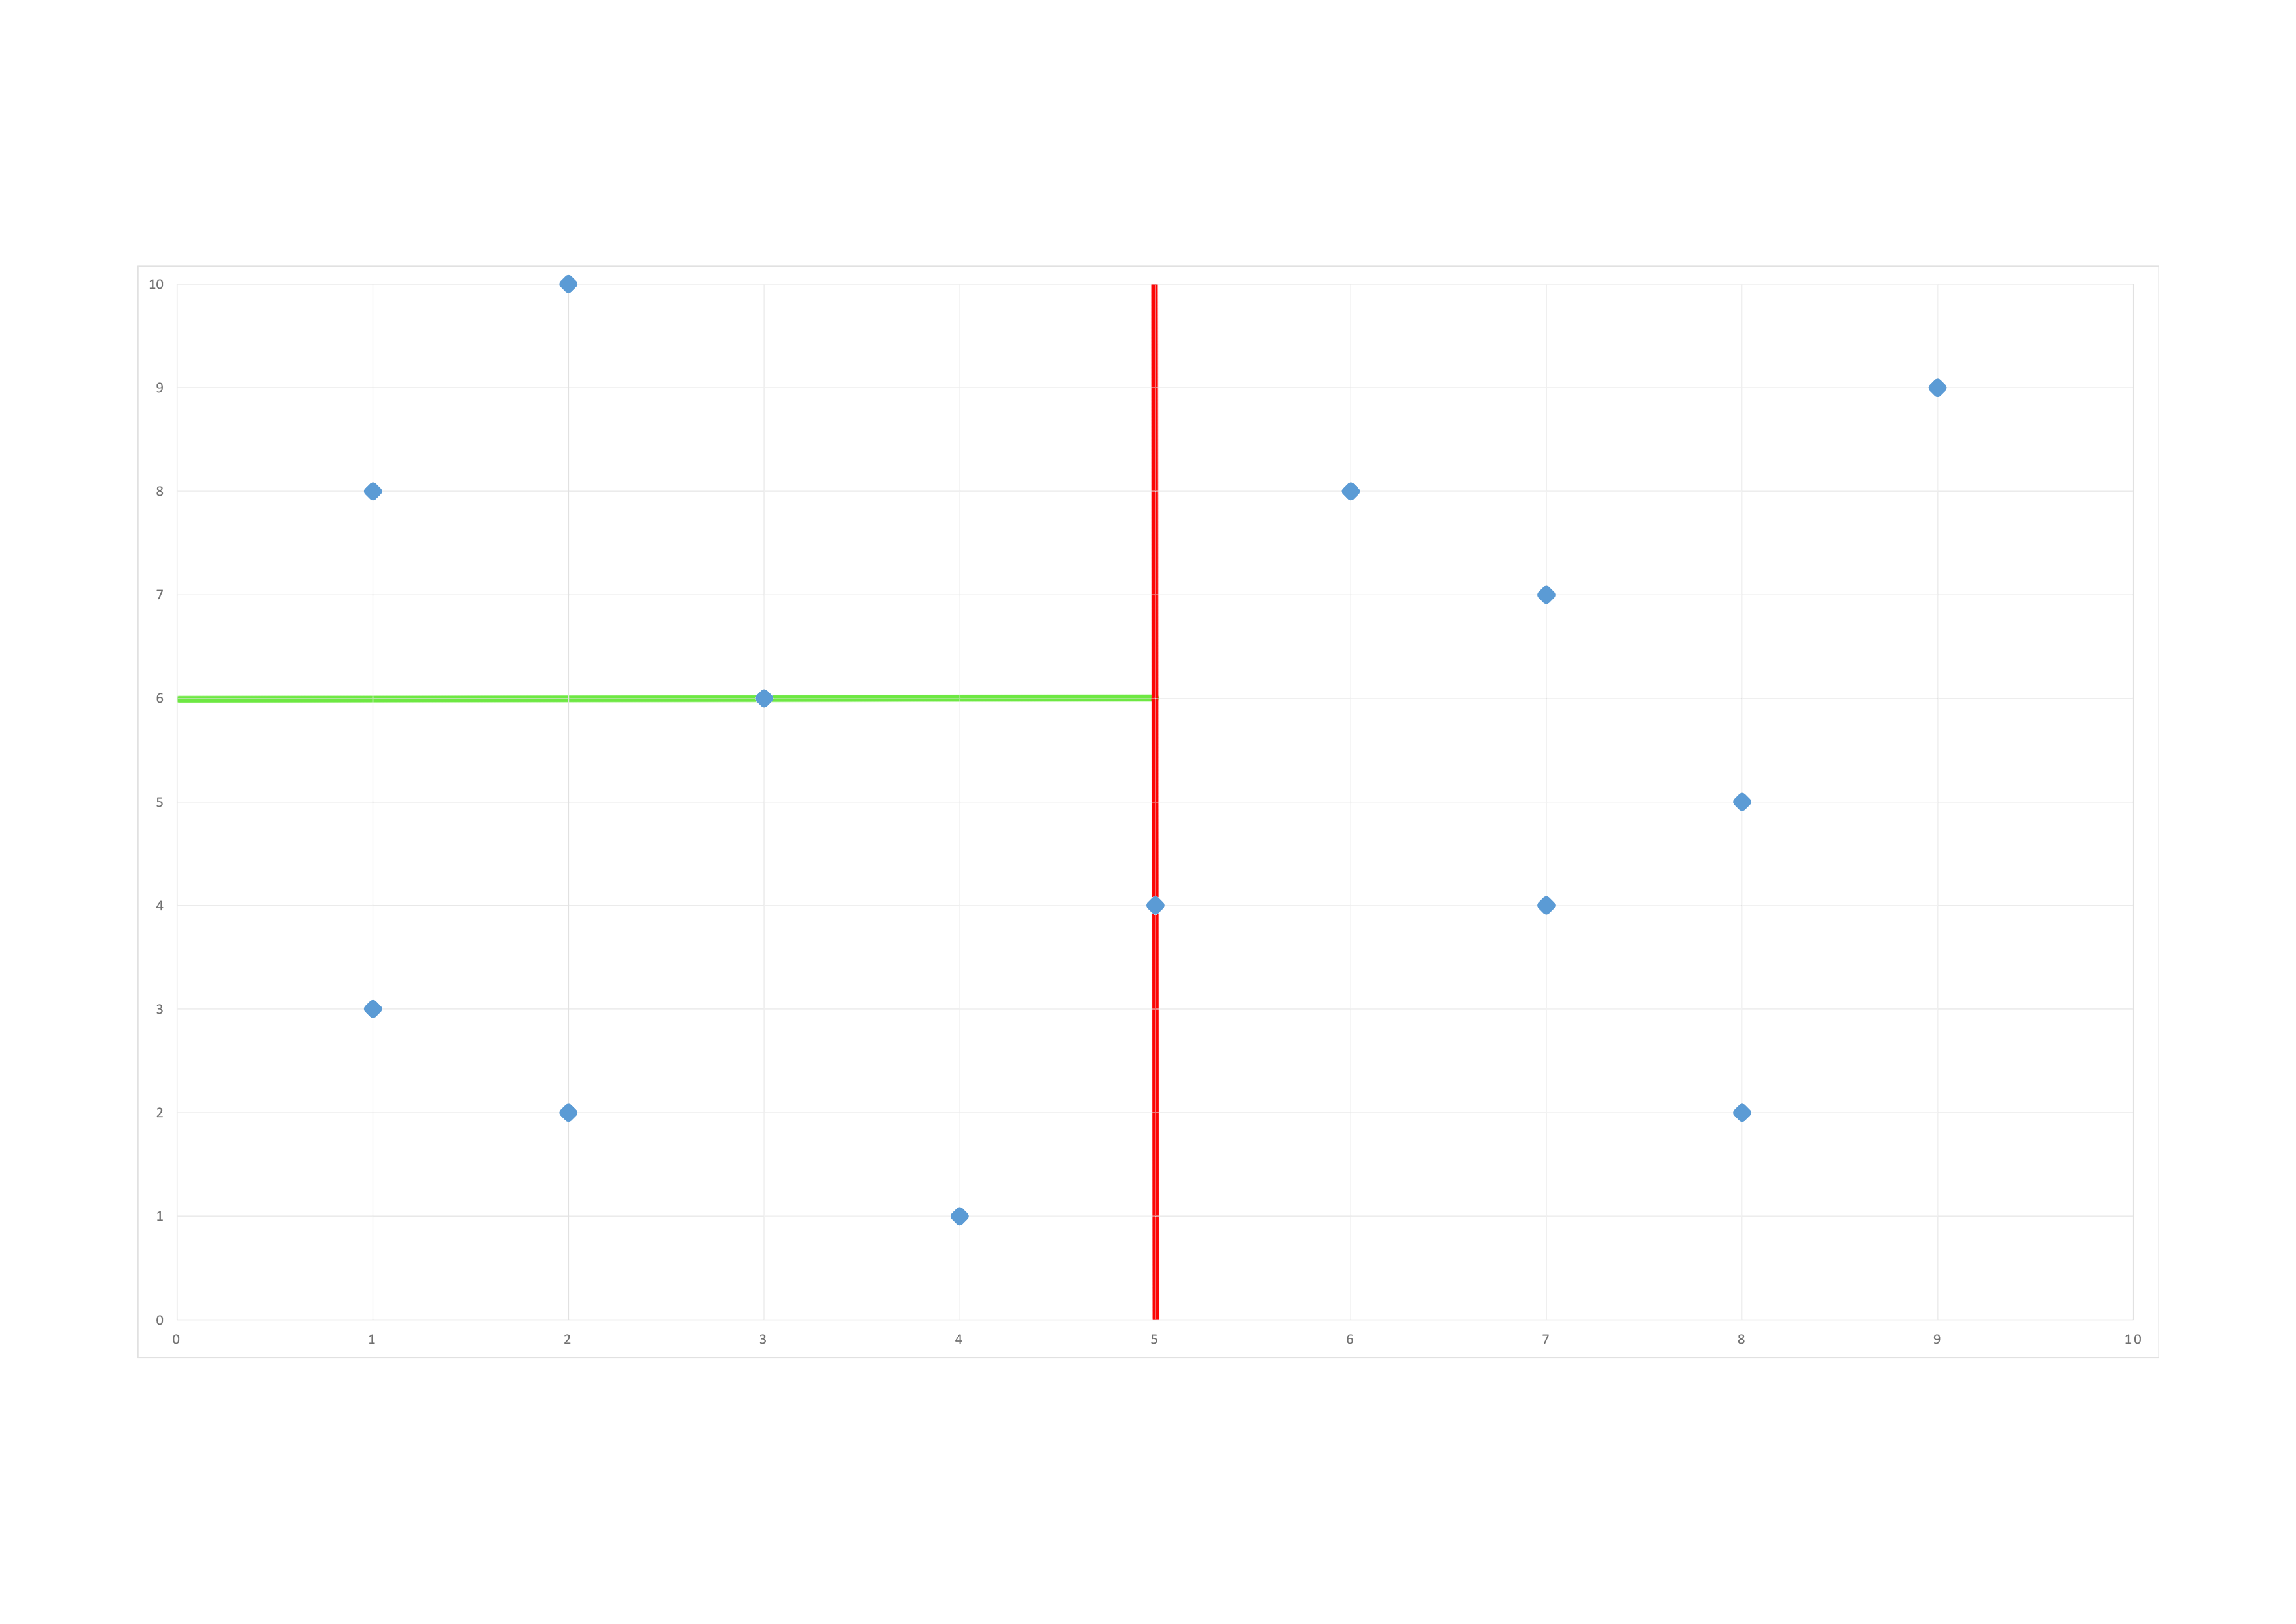
\includegraphics[width=.7\textwidth]{figures/split2.png}}
    \only<3>{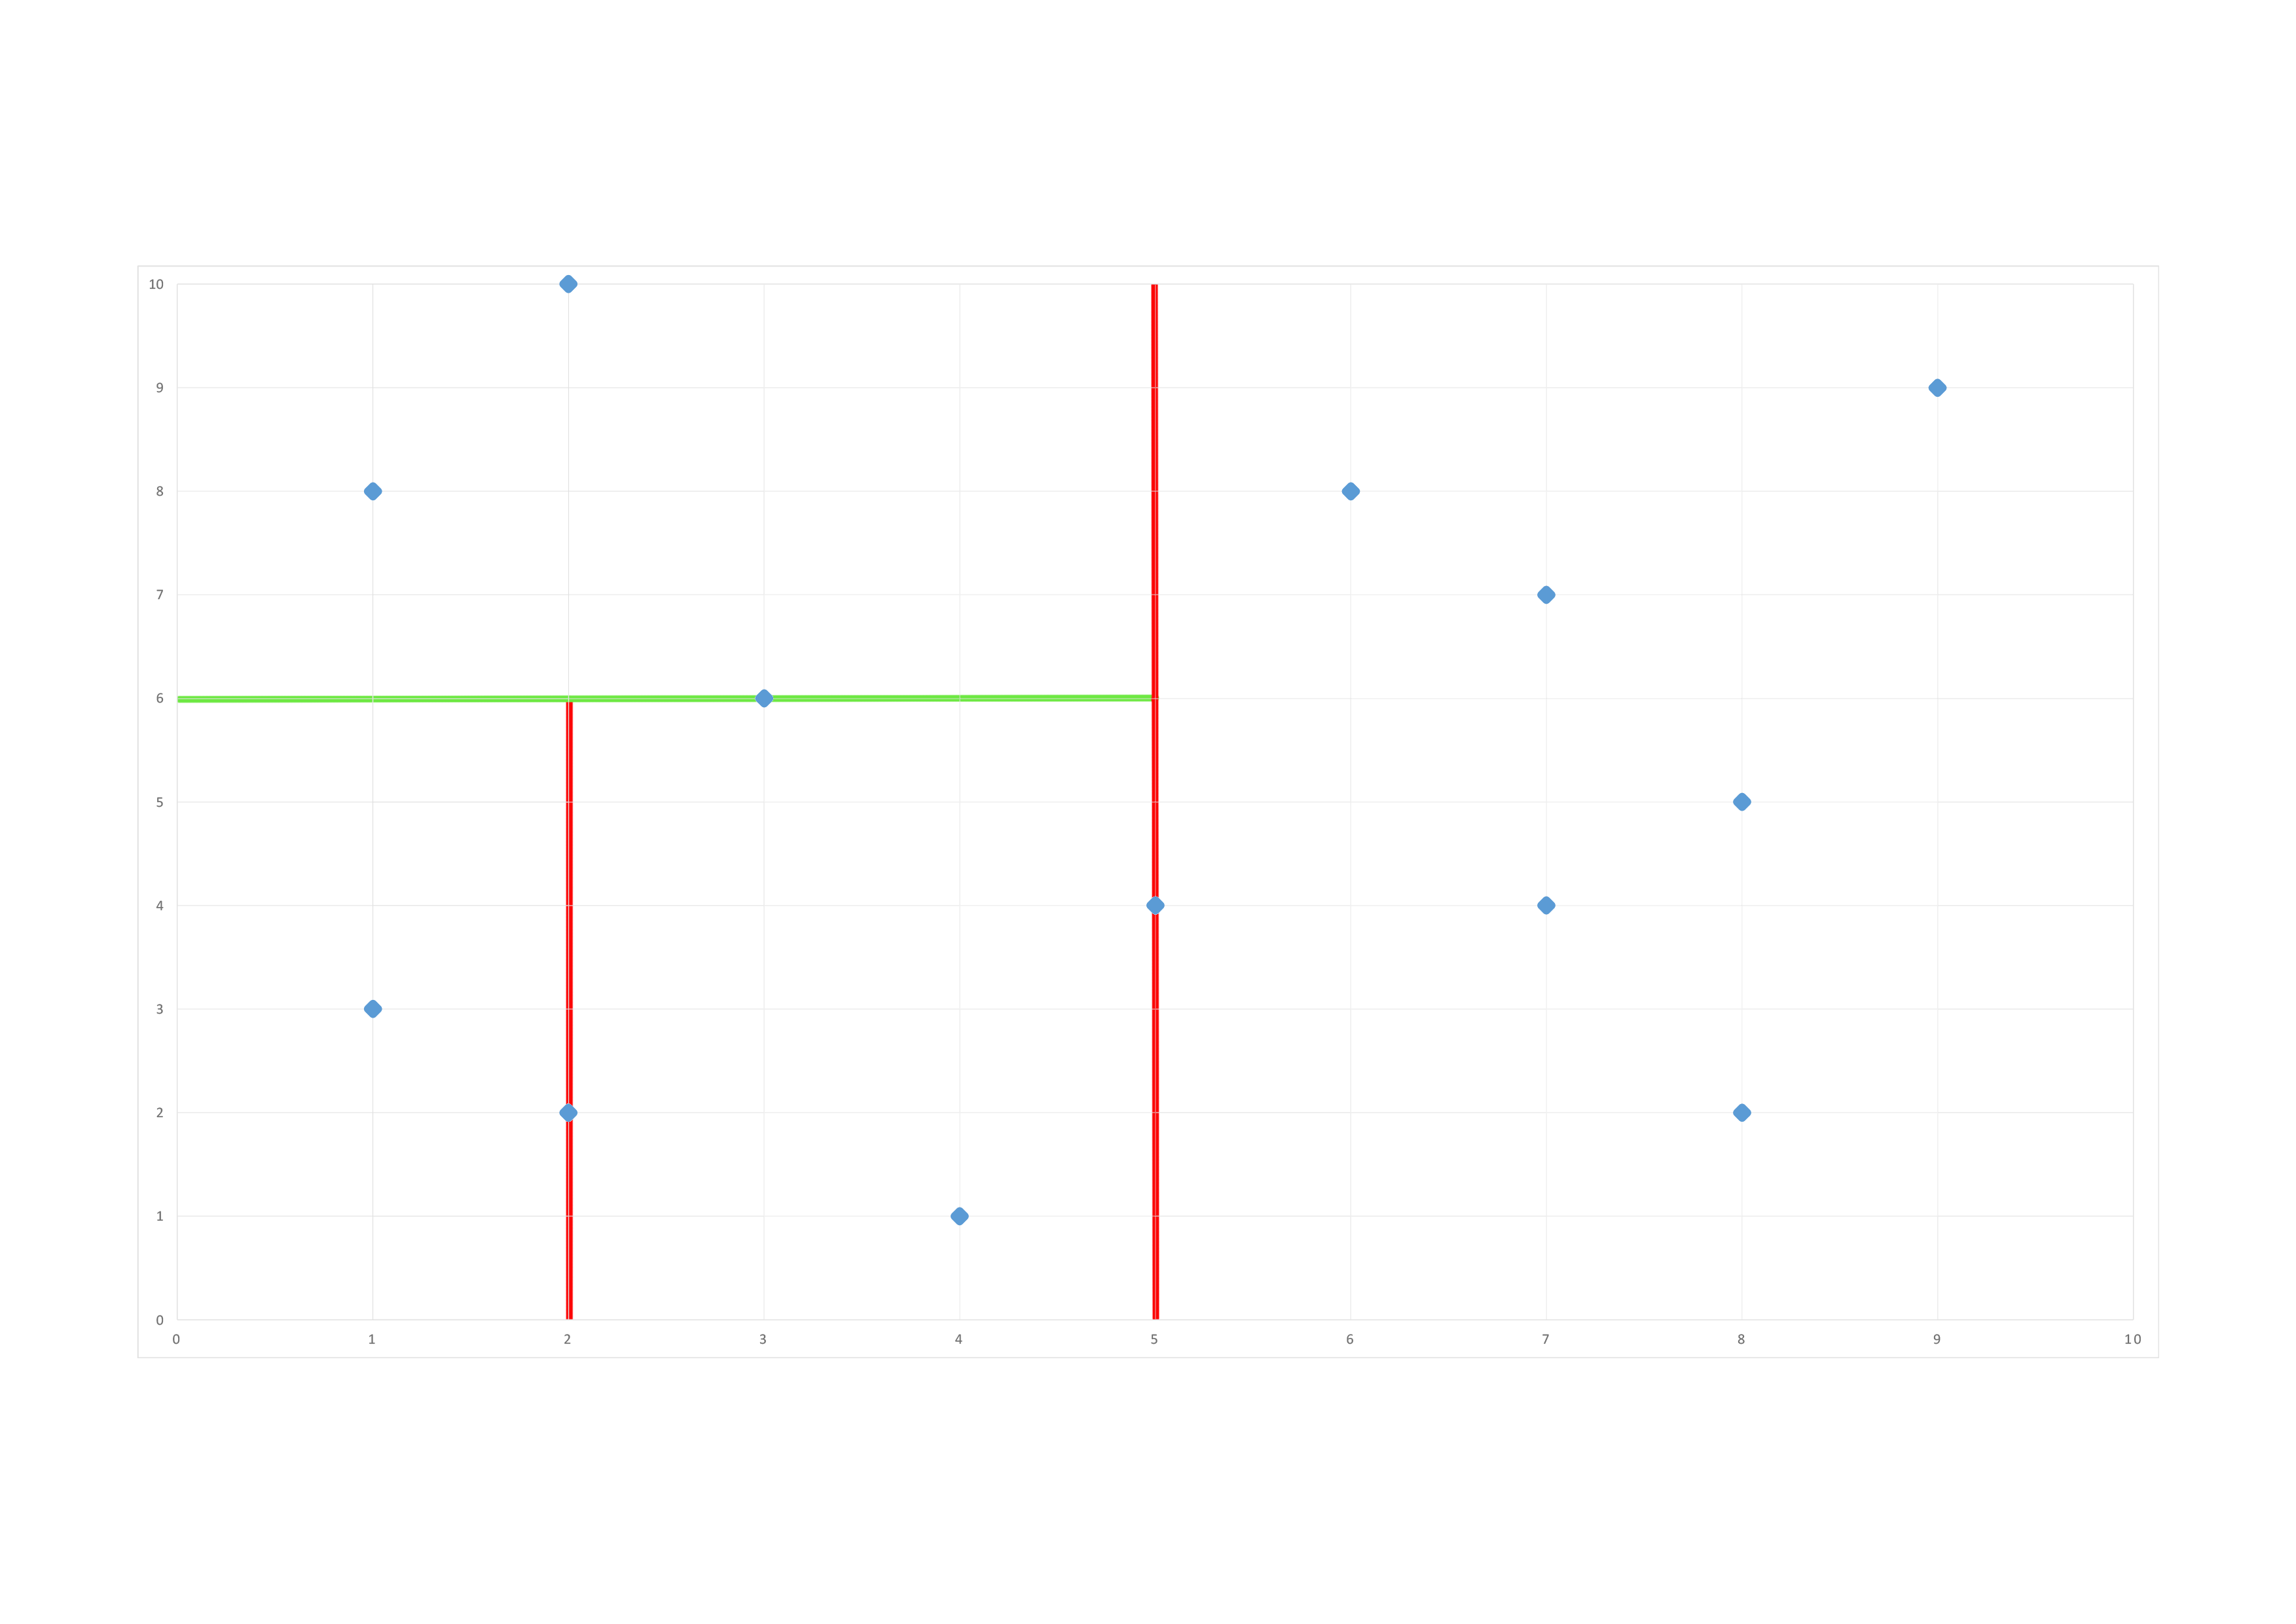
\includegraphics[width=.7\textwidth]{figures/split3.png}}
    \only<4>{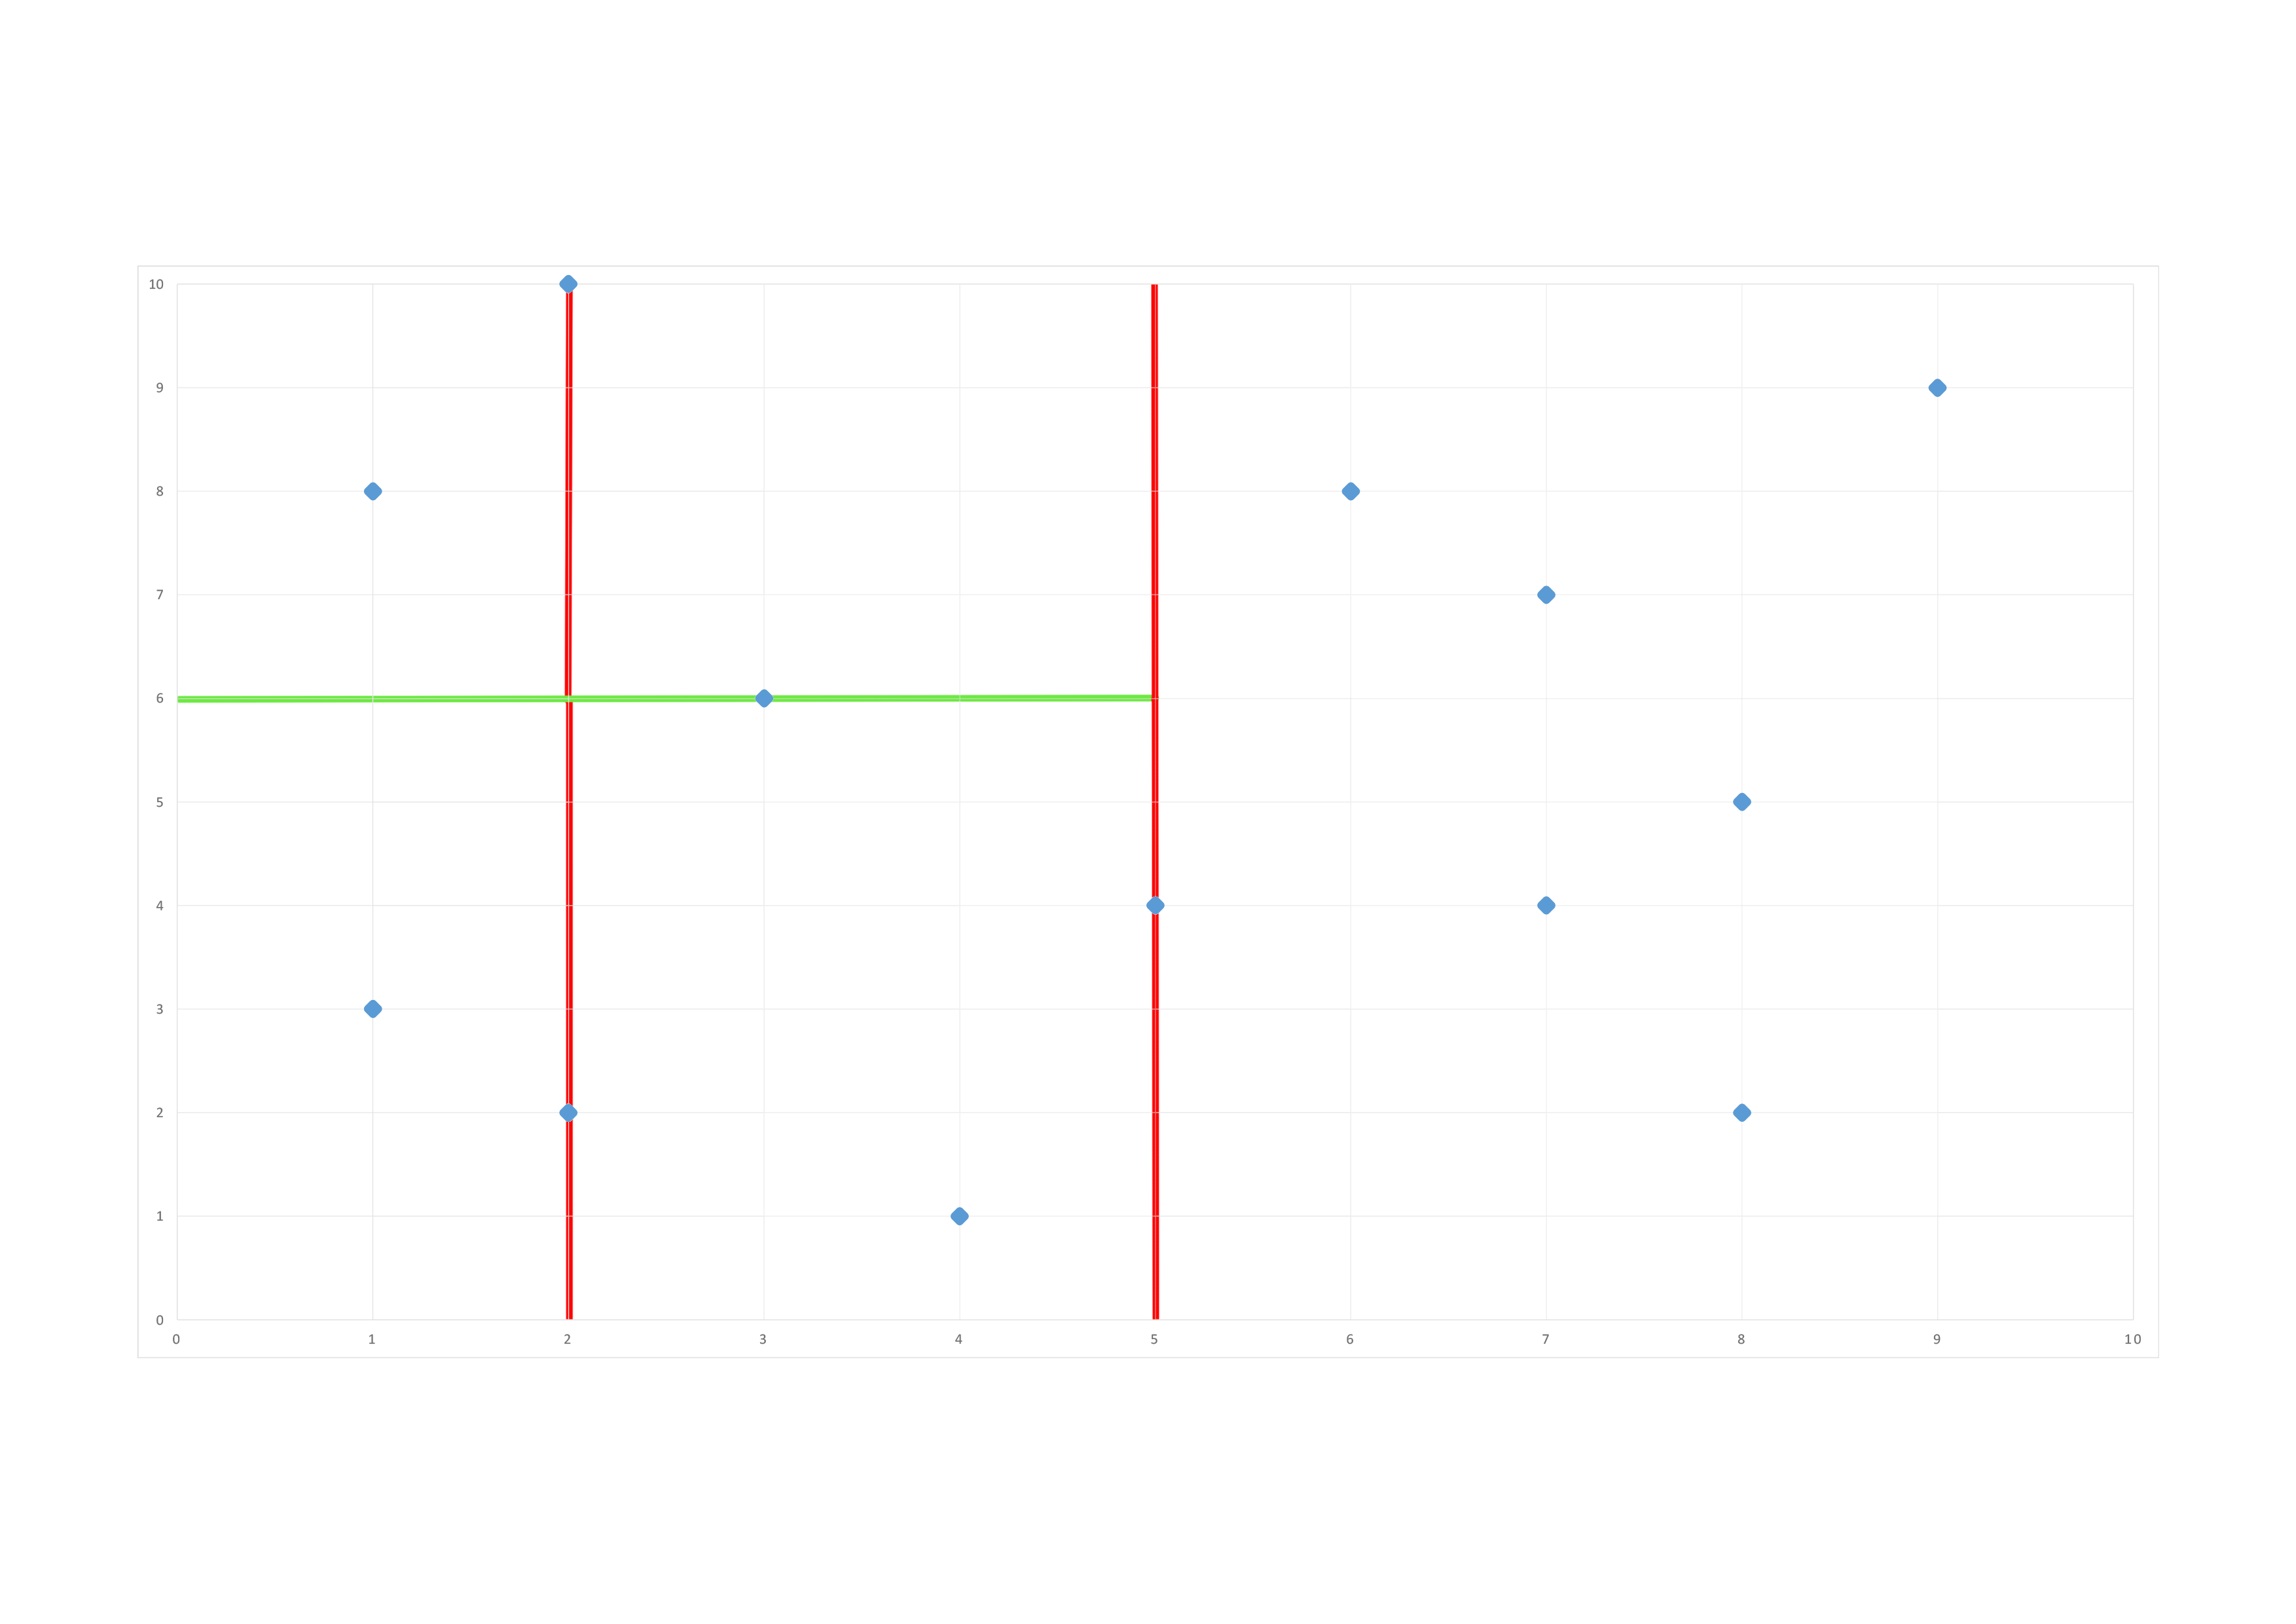
\includegraphics[width=.7\textwidth]{figures/split4.png}}
    \only<5>{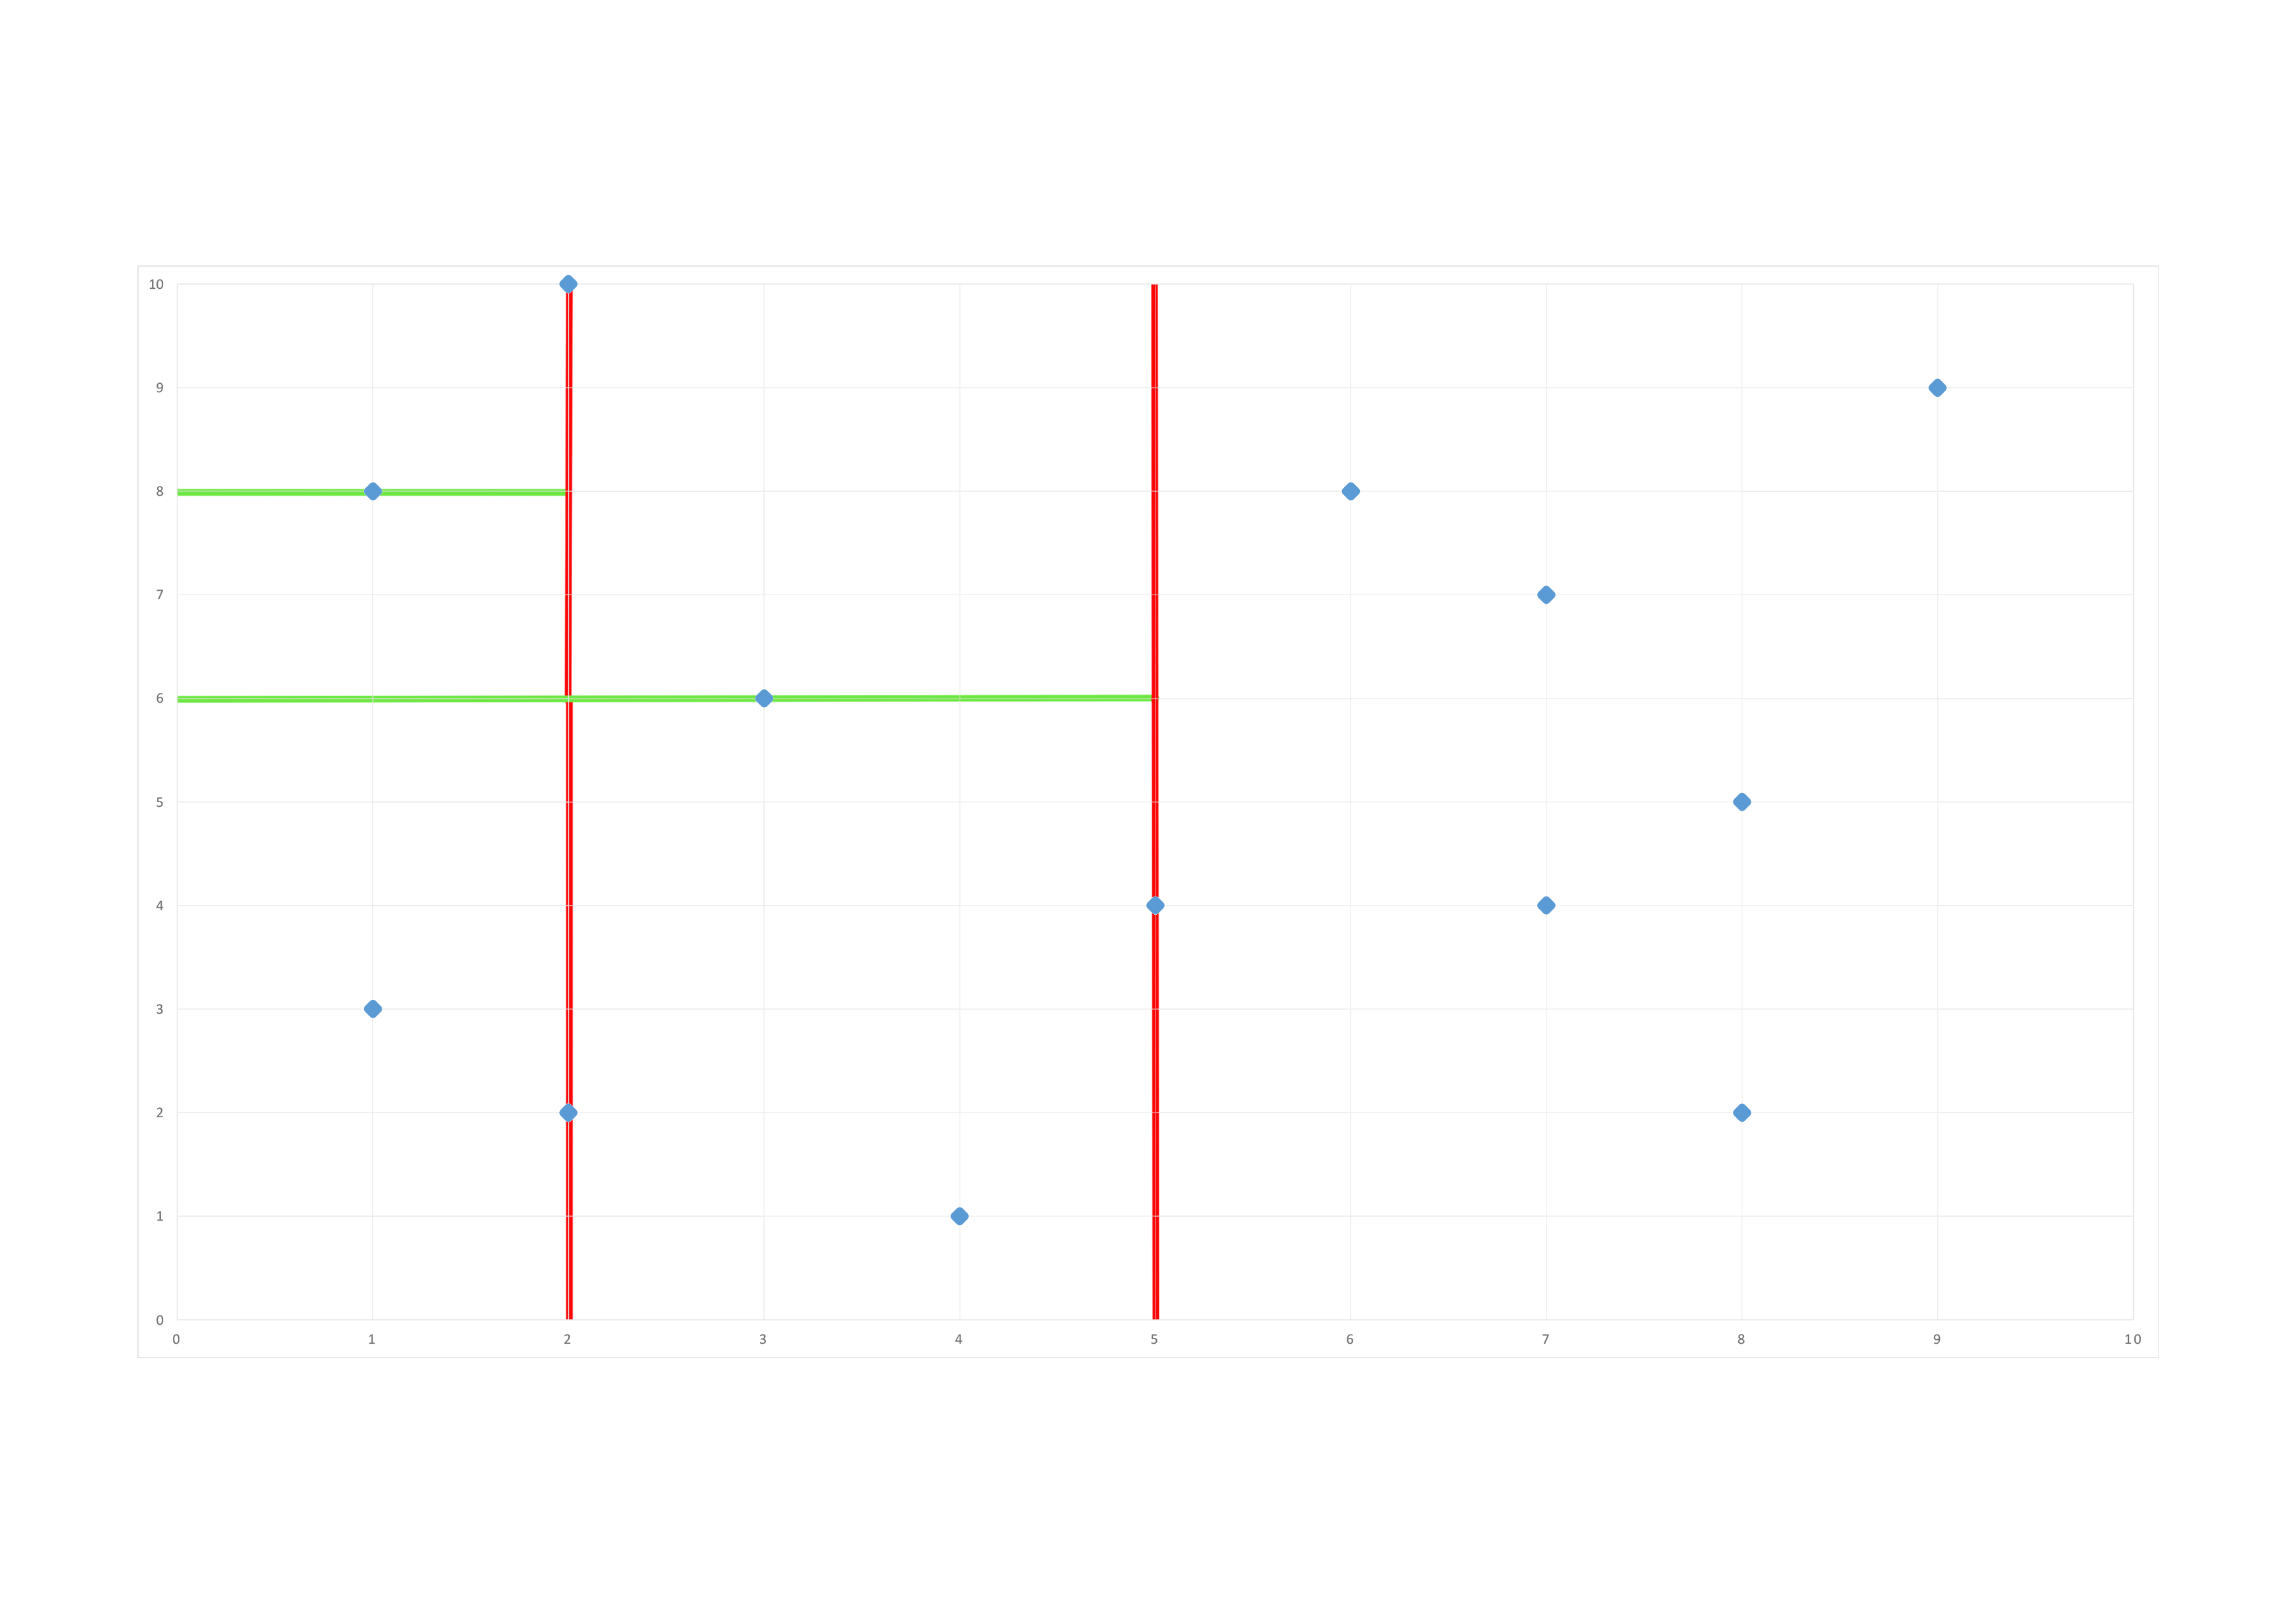
\includegraphics[width=.7\textwidth]{figures/split5.png}}
    \only<6>{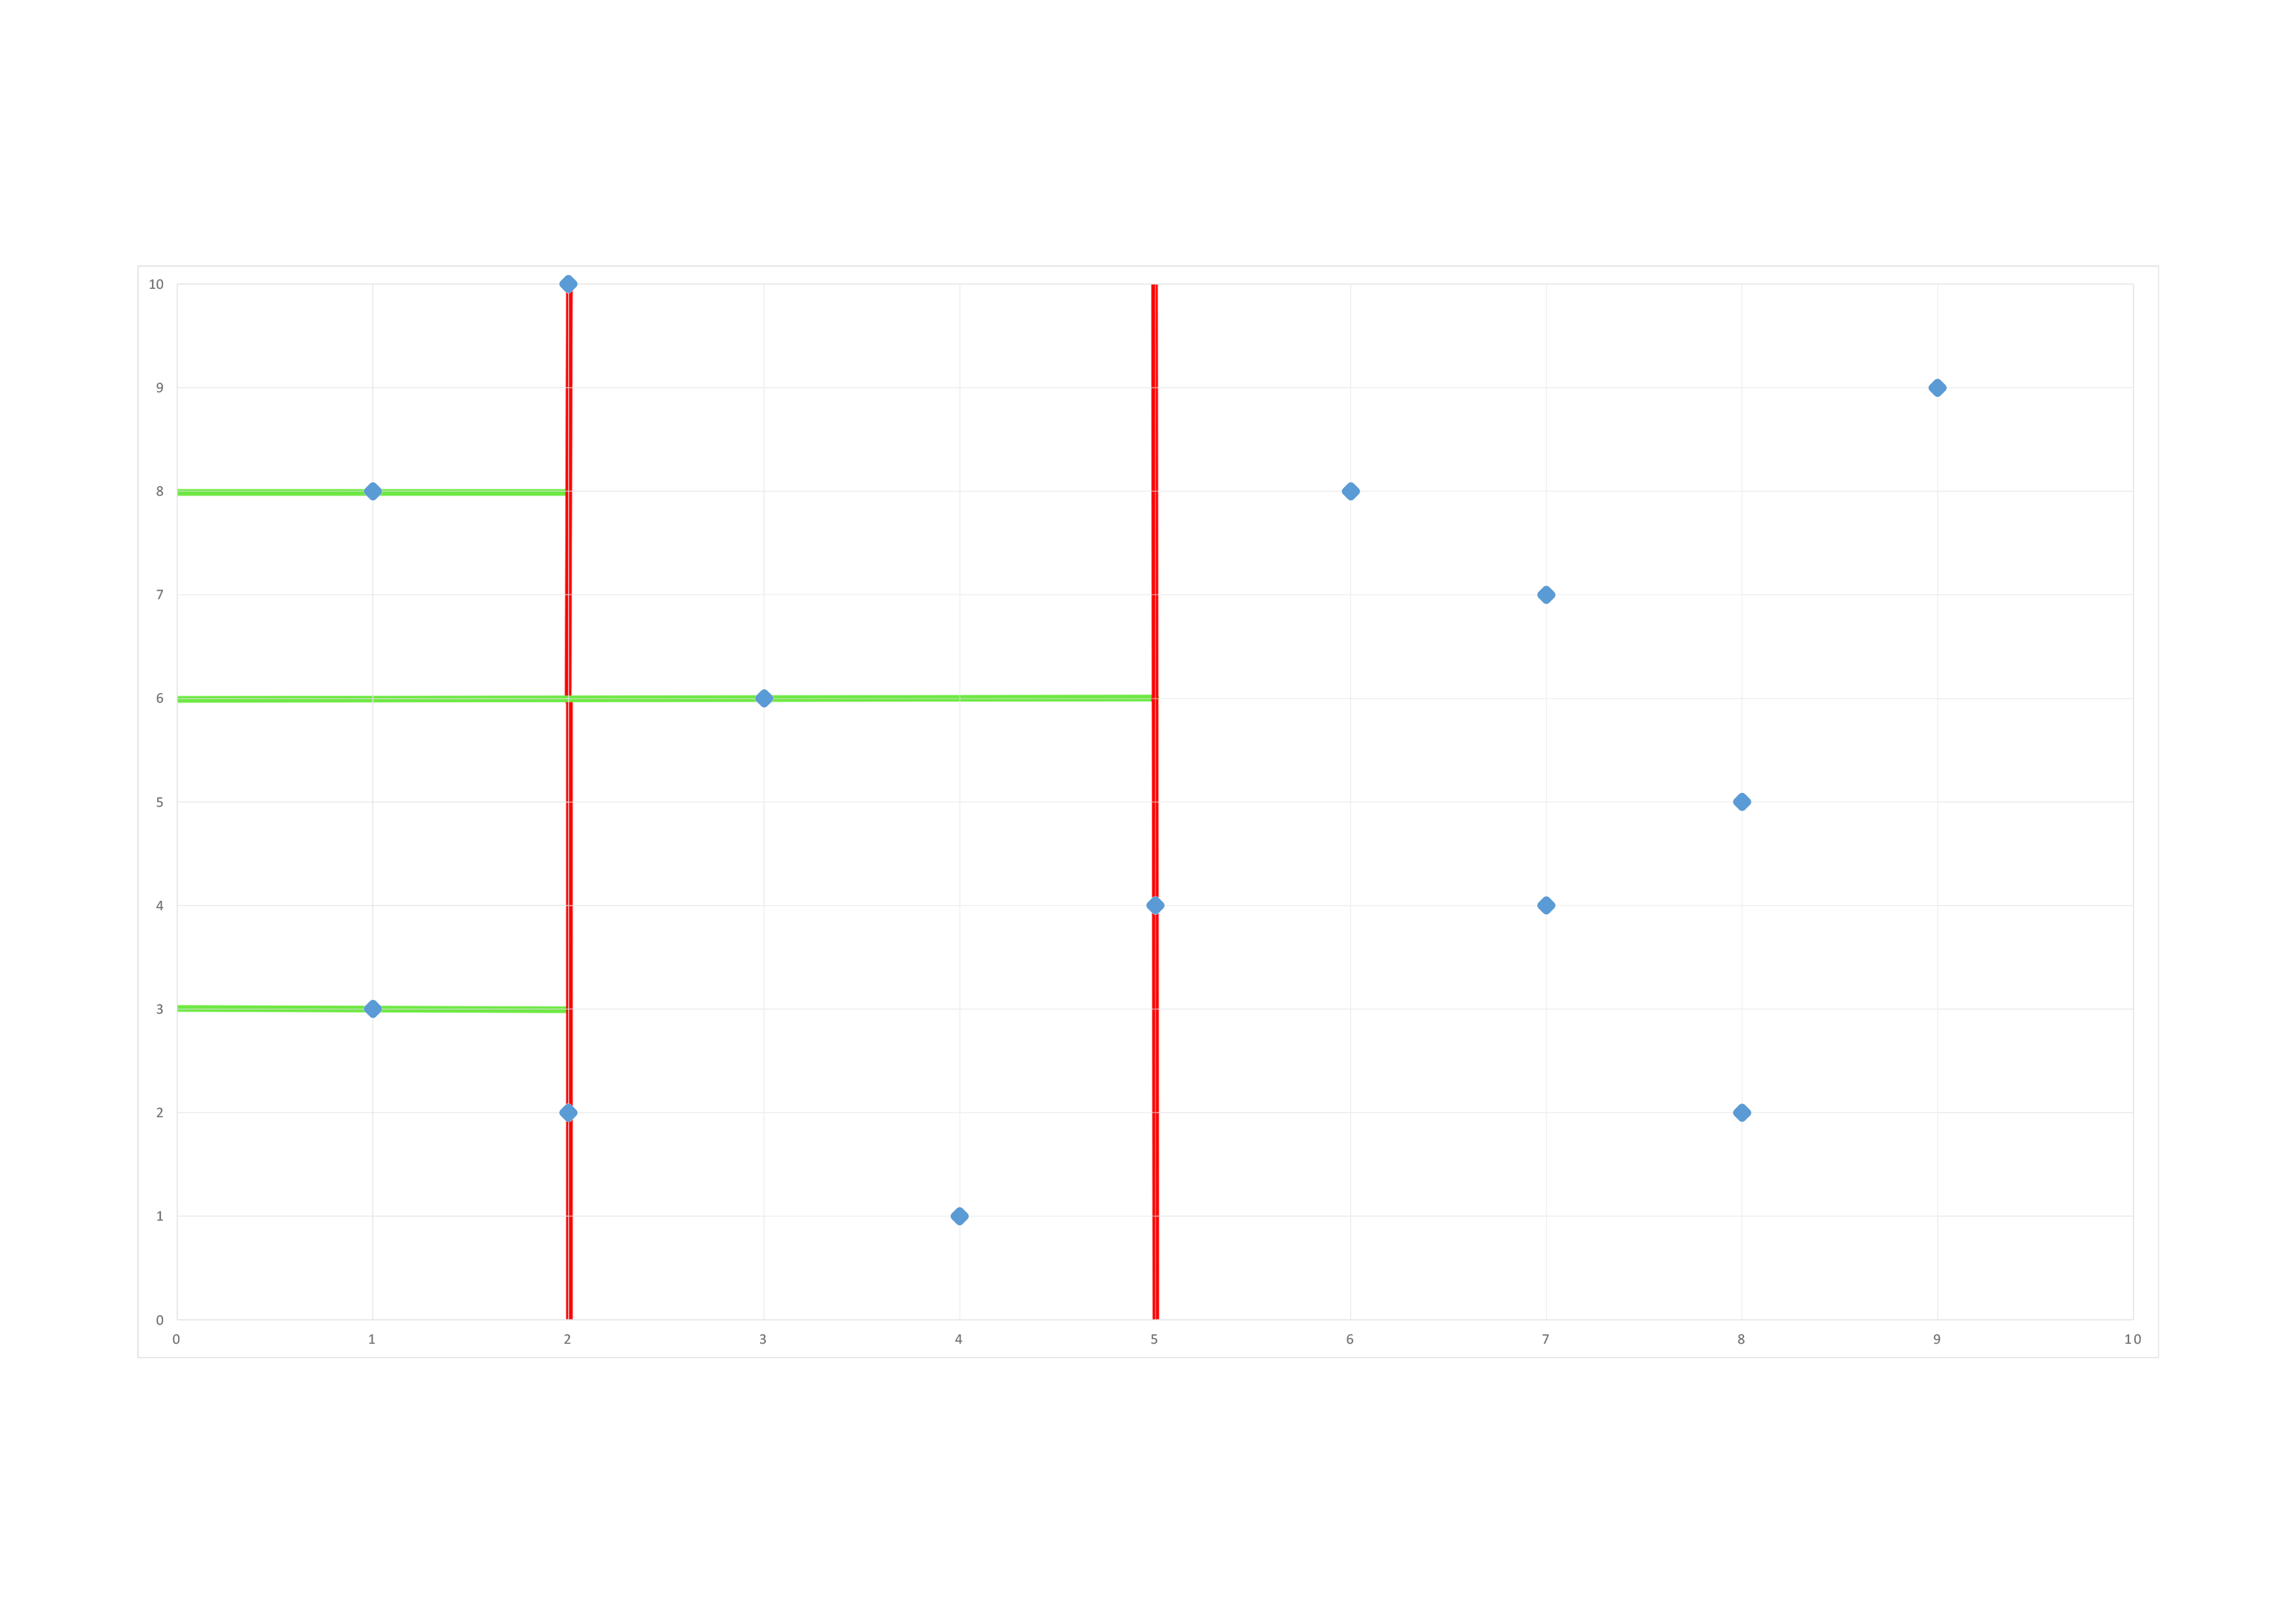
\includegraphics[width=.7\textwidth]{figures/split6.png}}
    \only<7>{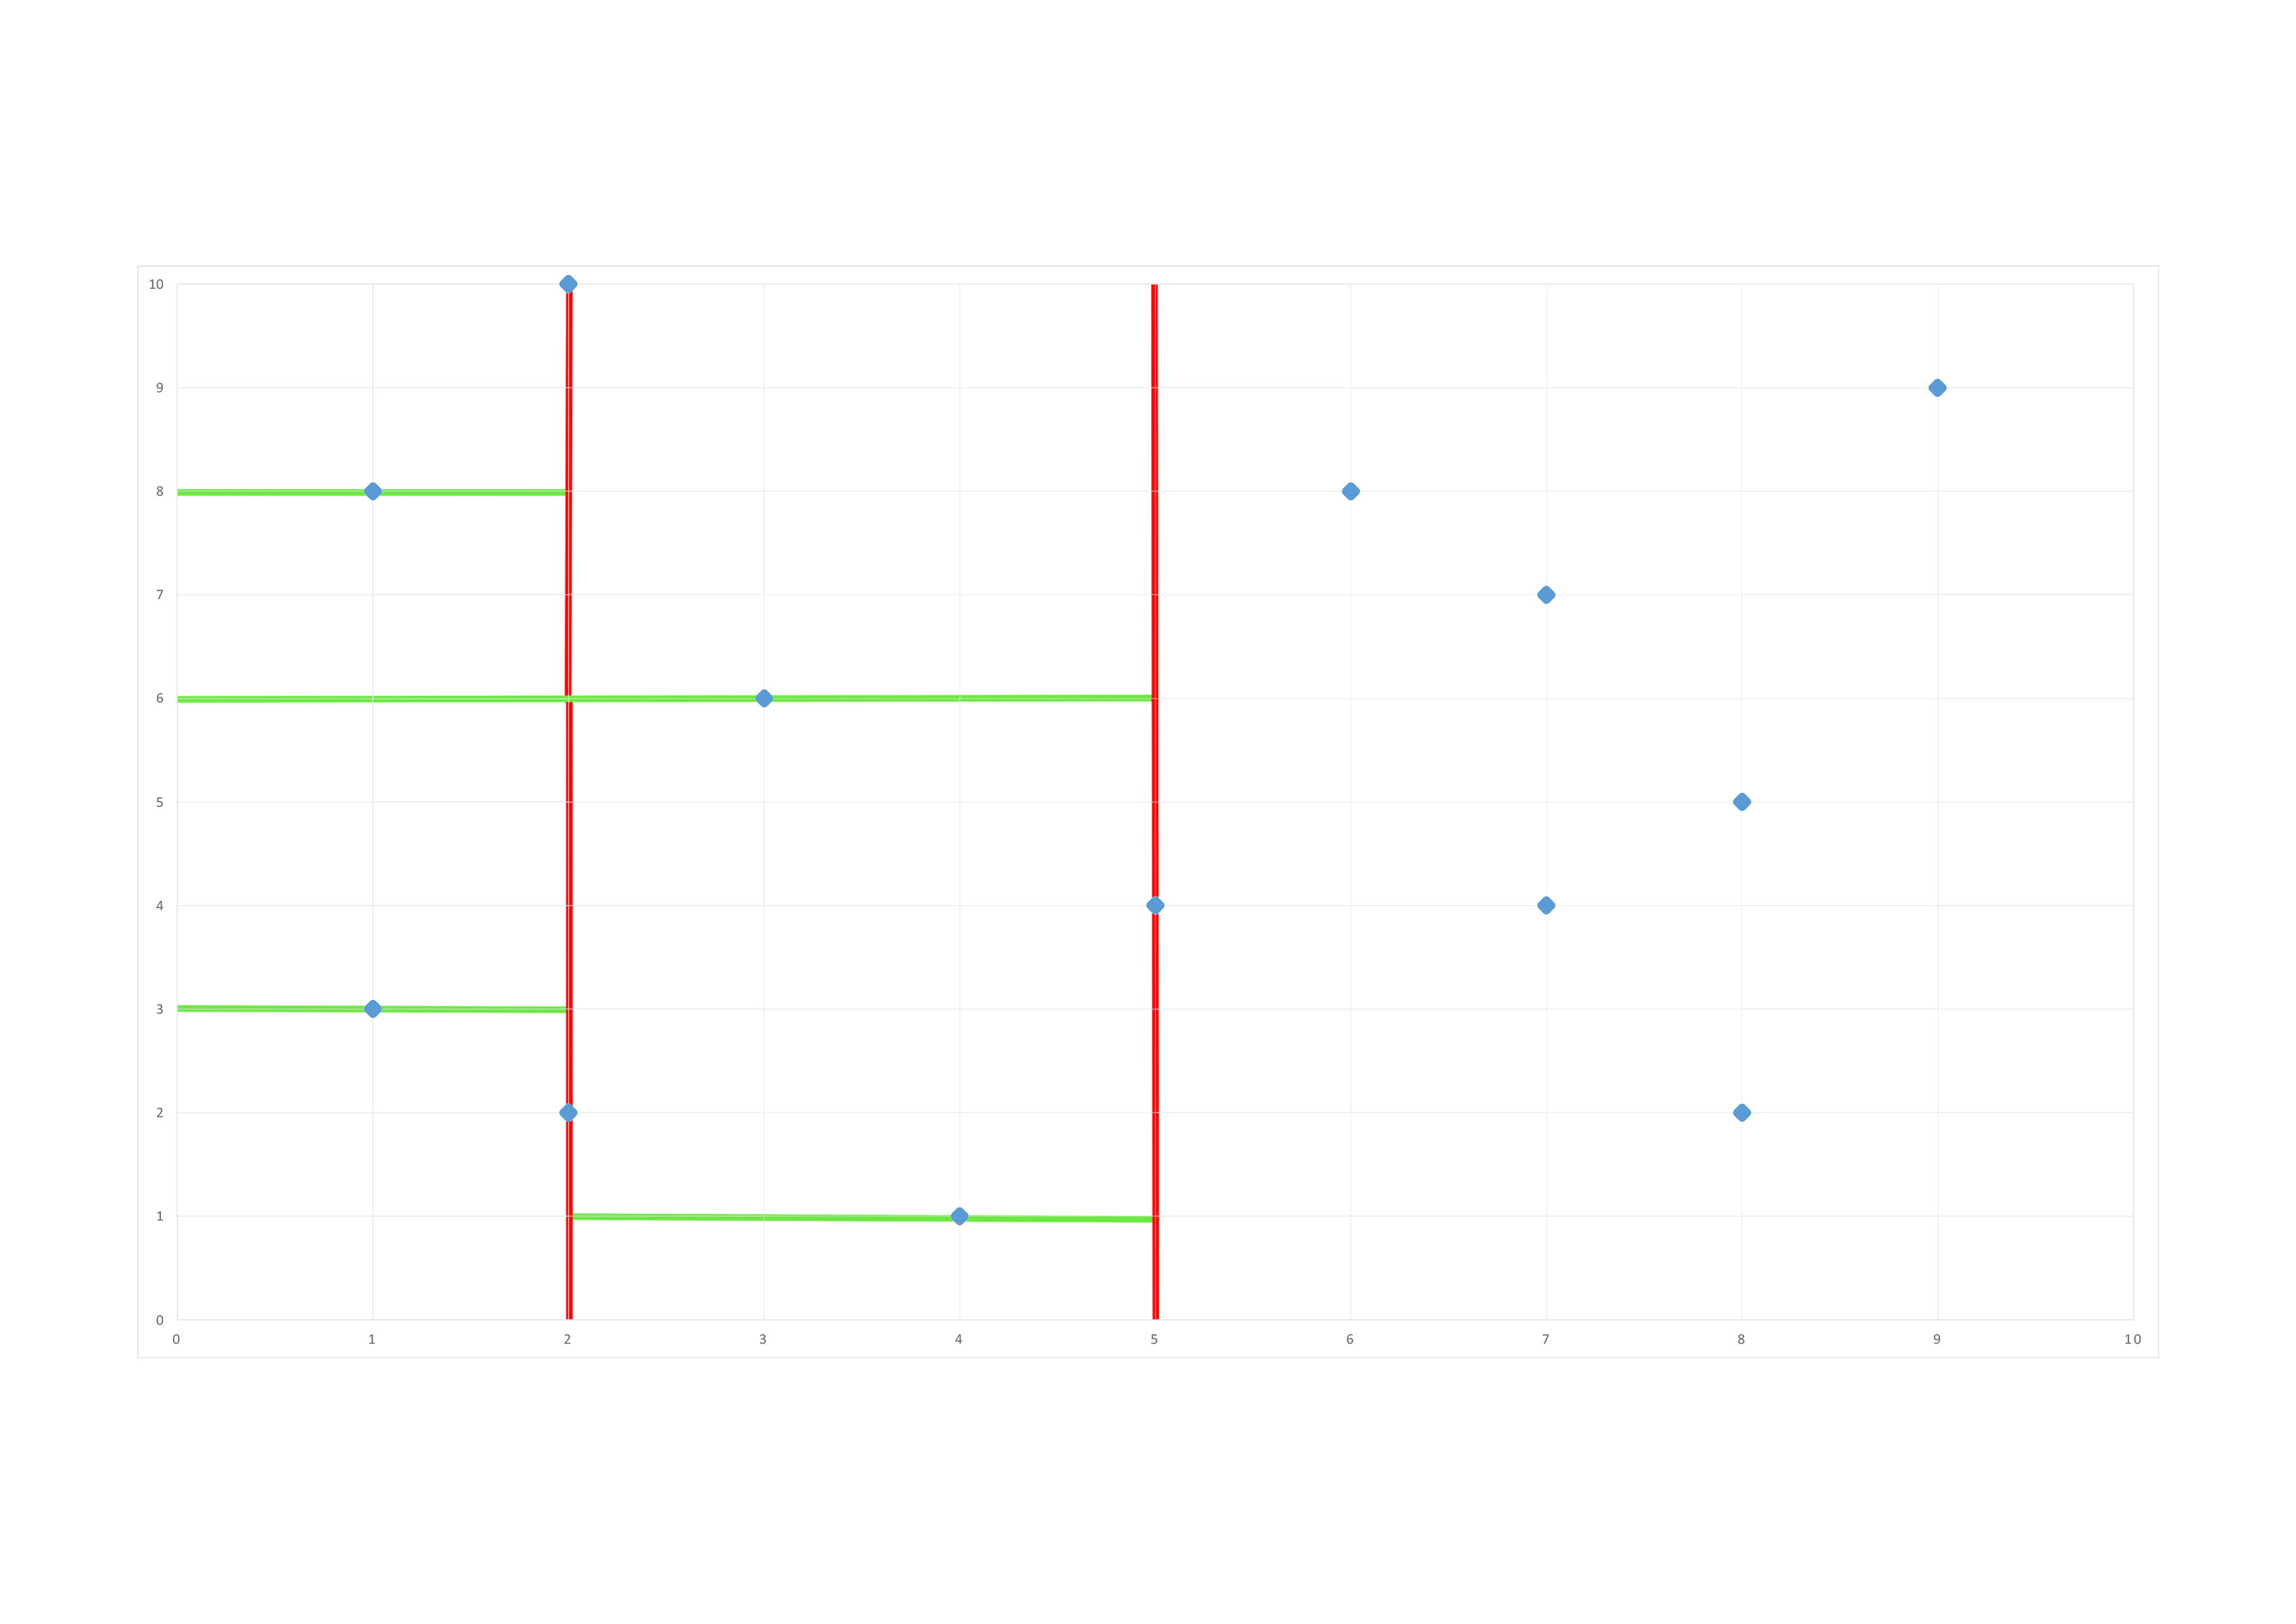
\includegraphics[width=.7\textwidth]{figures/split7.png}}
    \only<8>{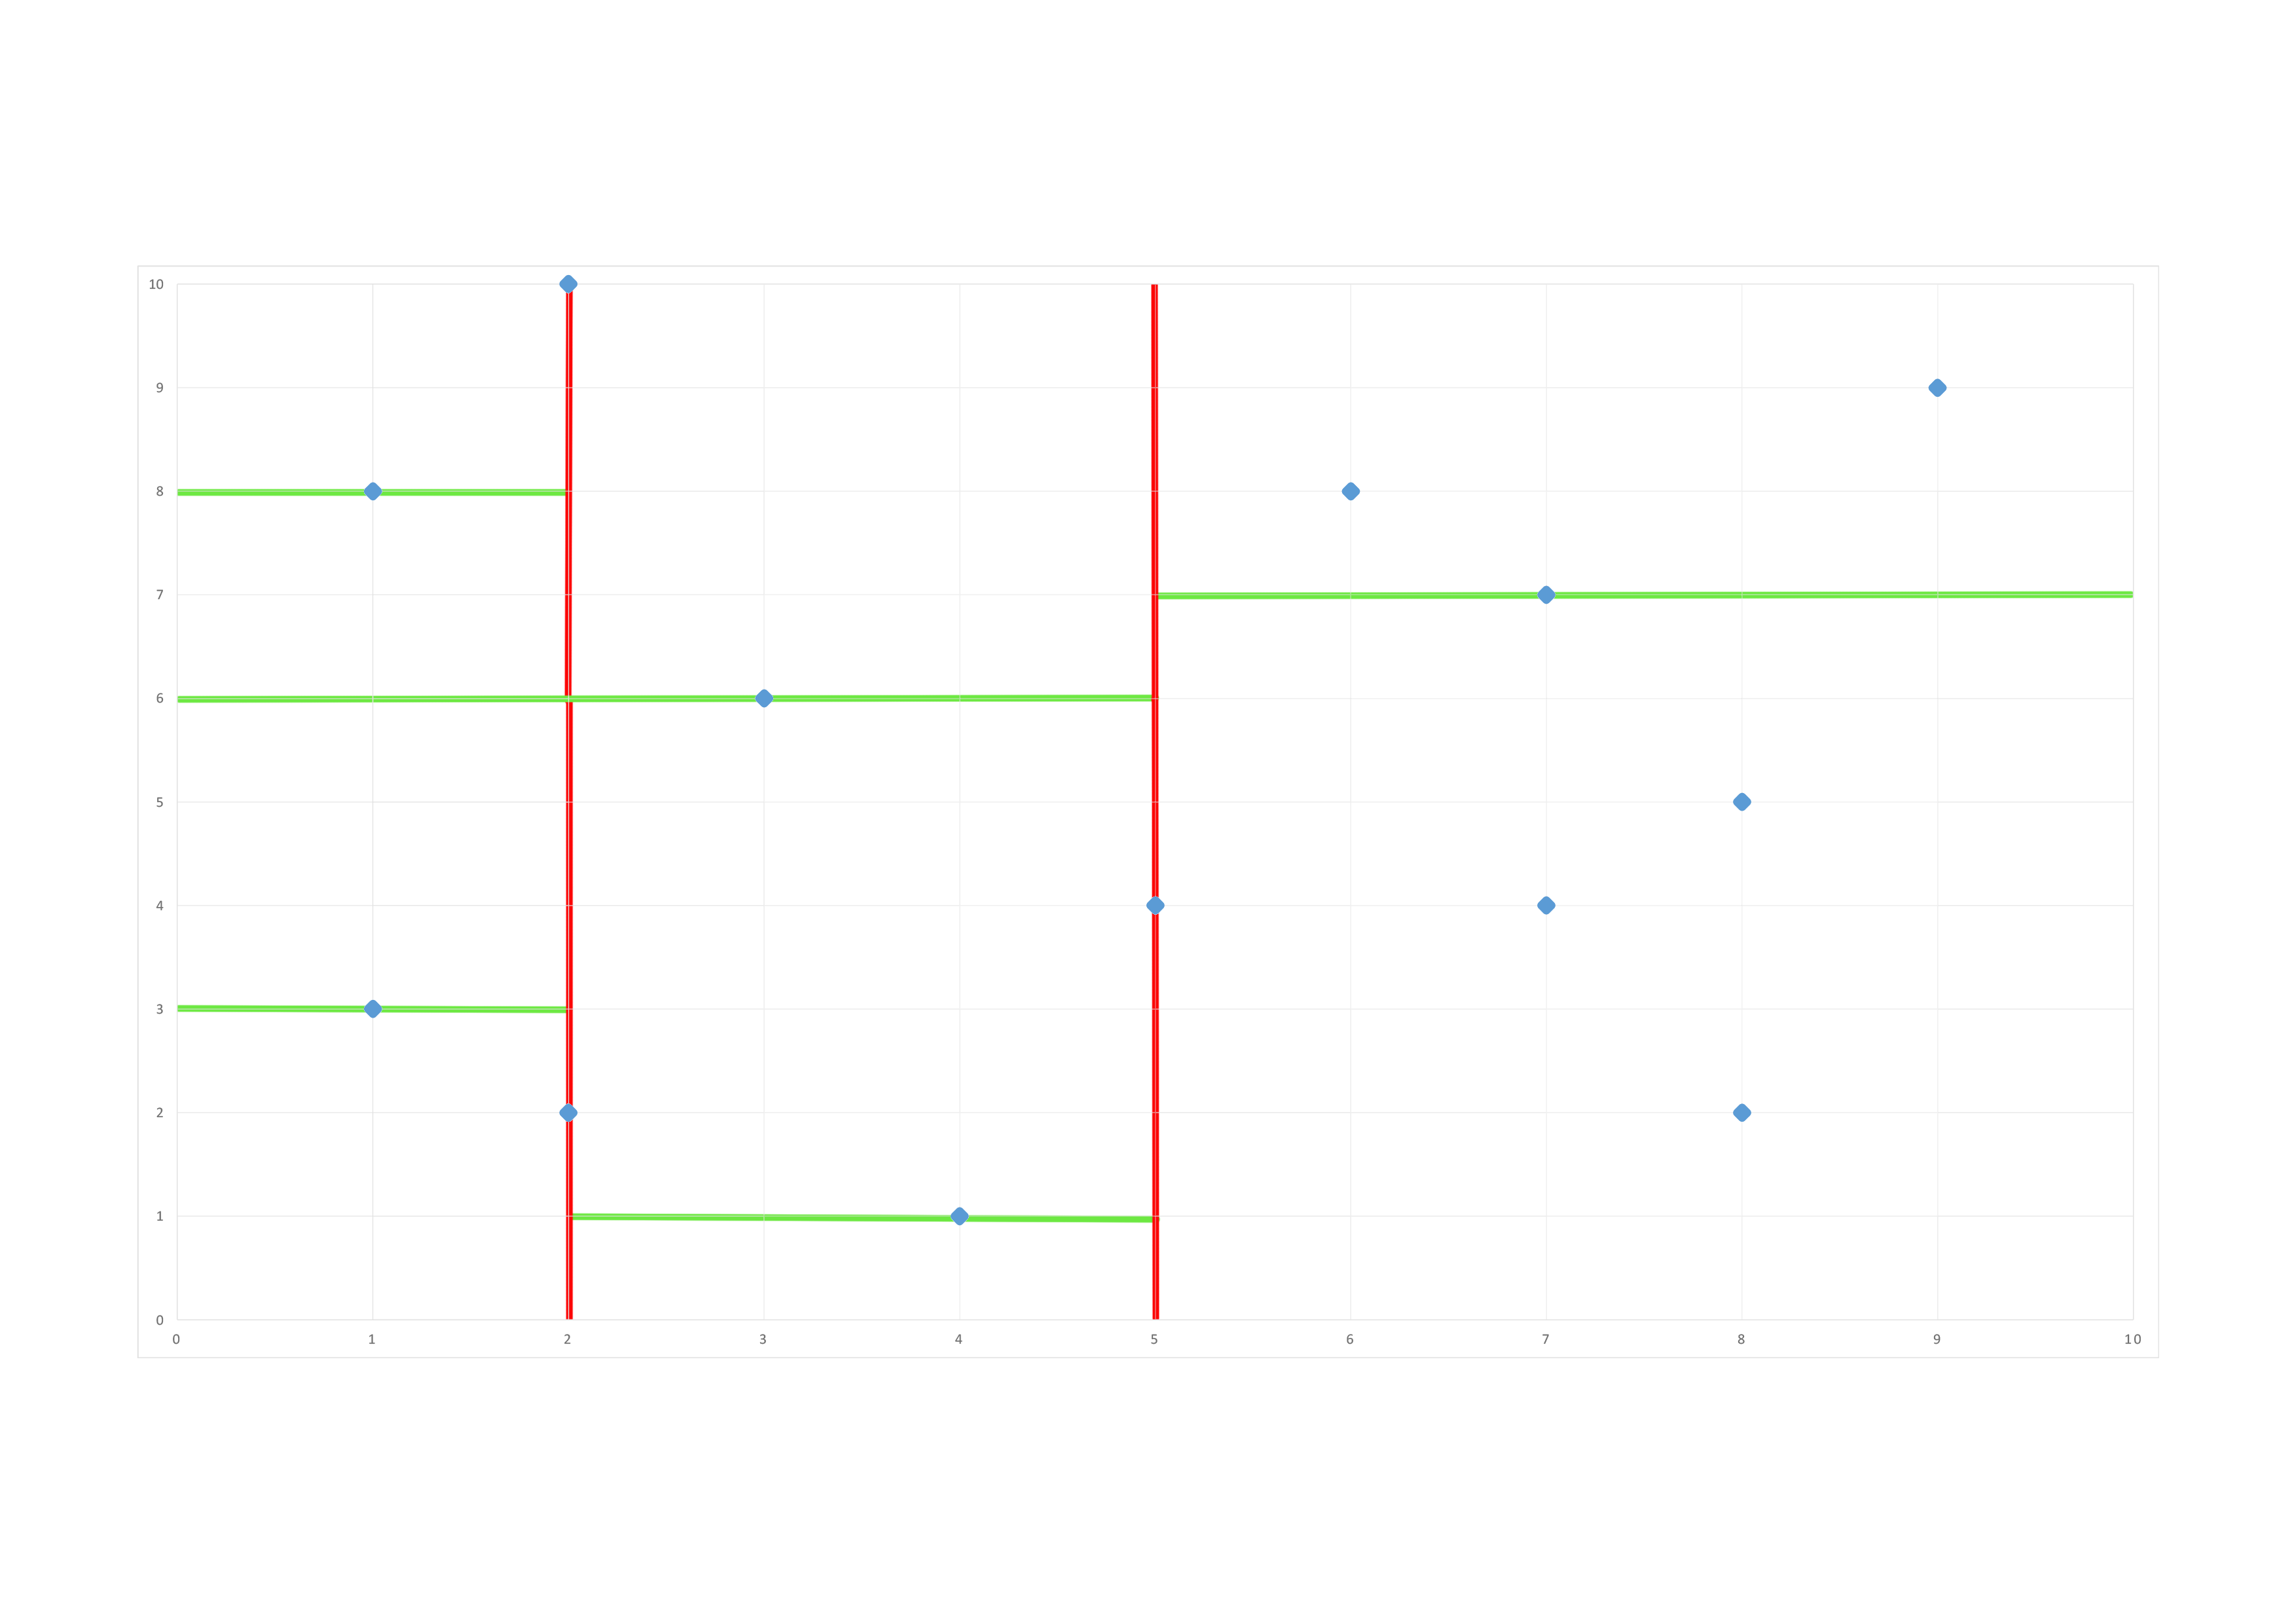
\includegraphics[width=.7\textwidth]{figures/split8.png}}
    \only<9>{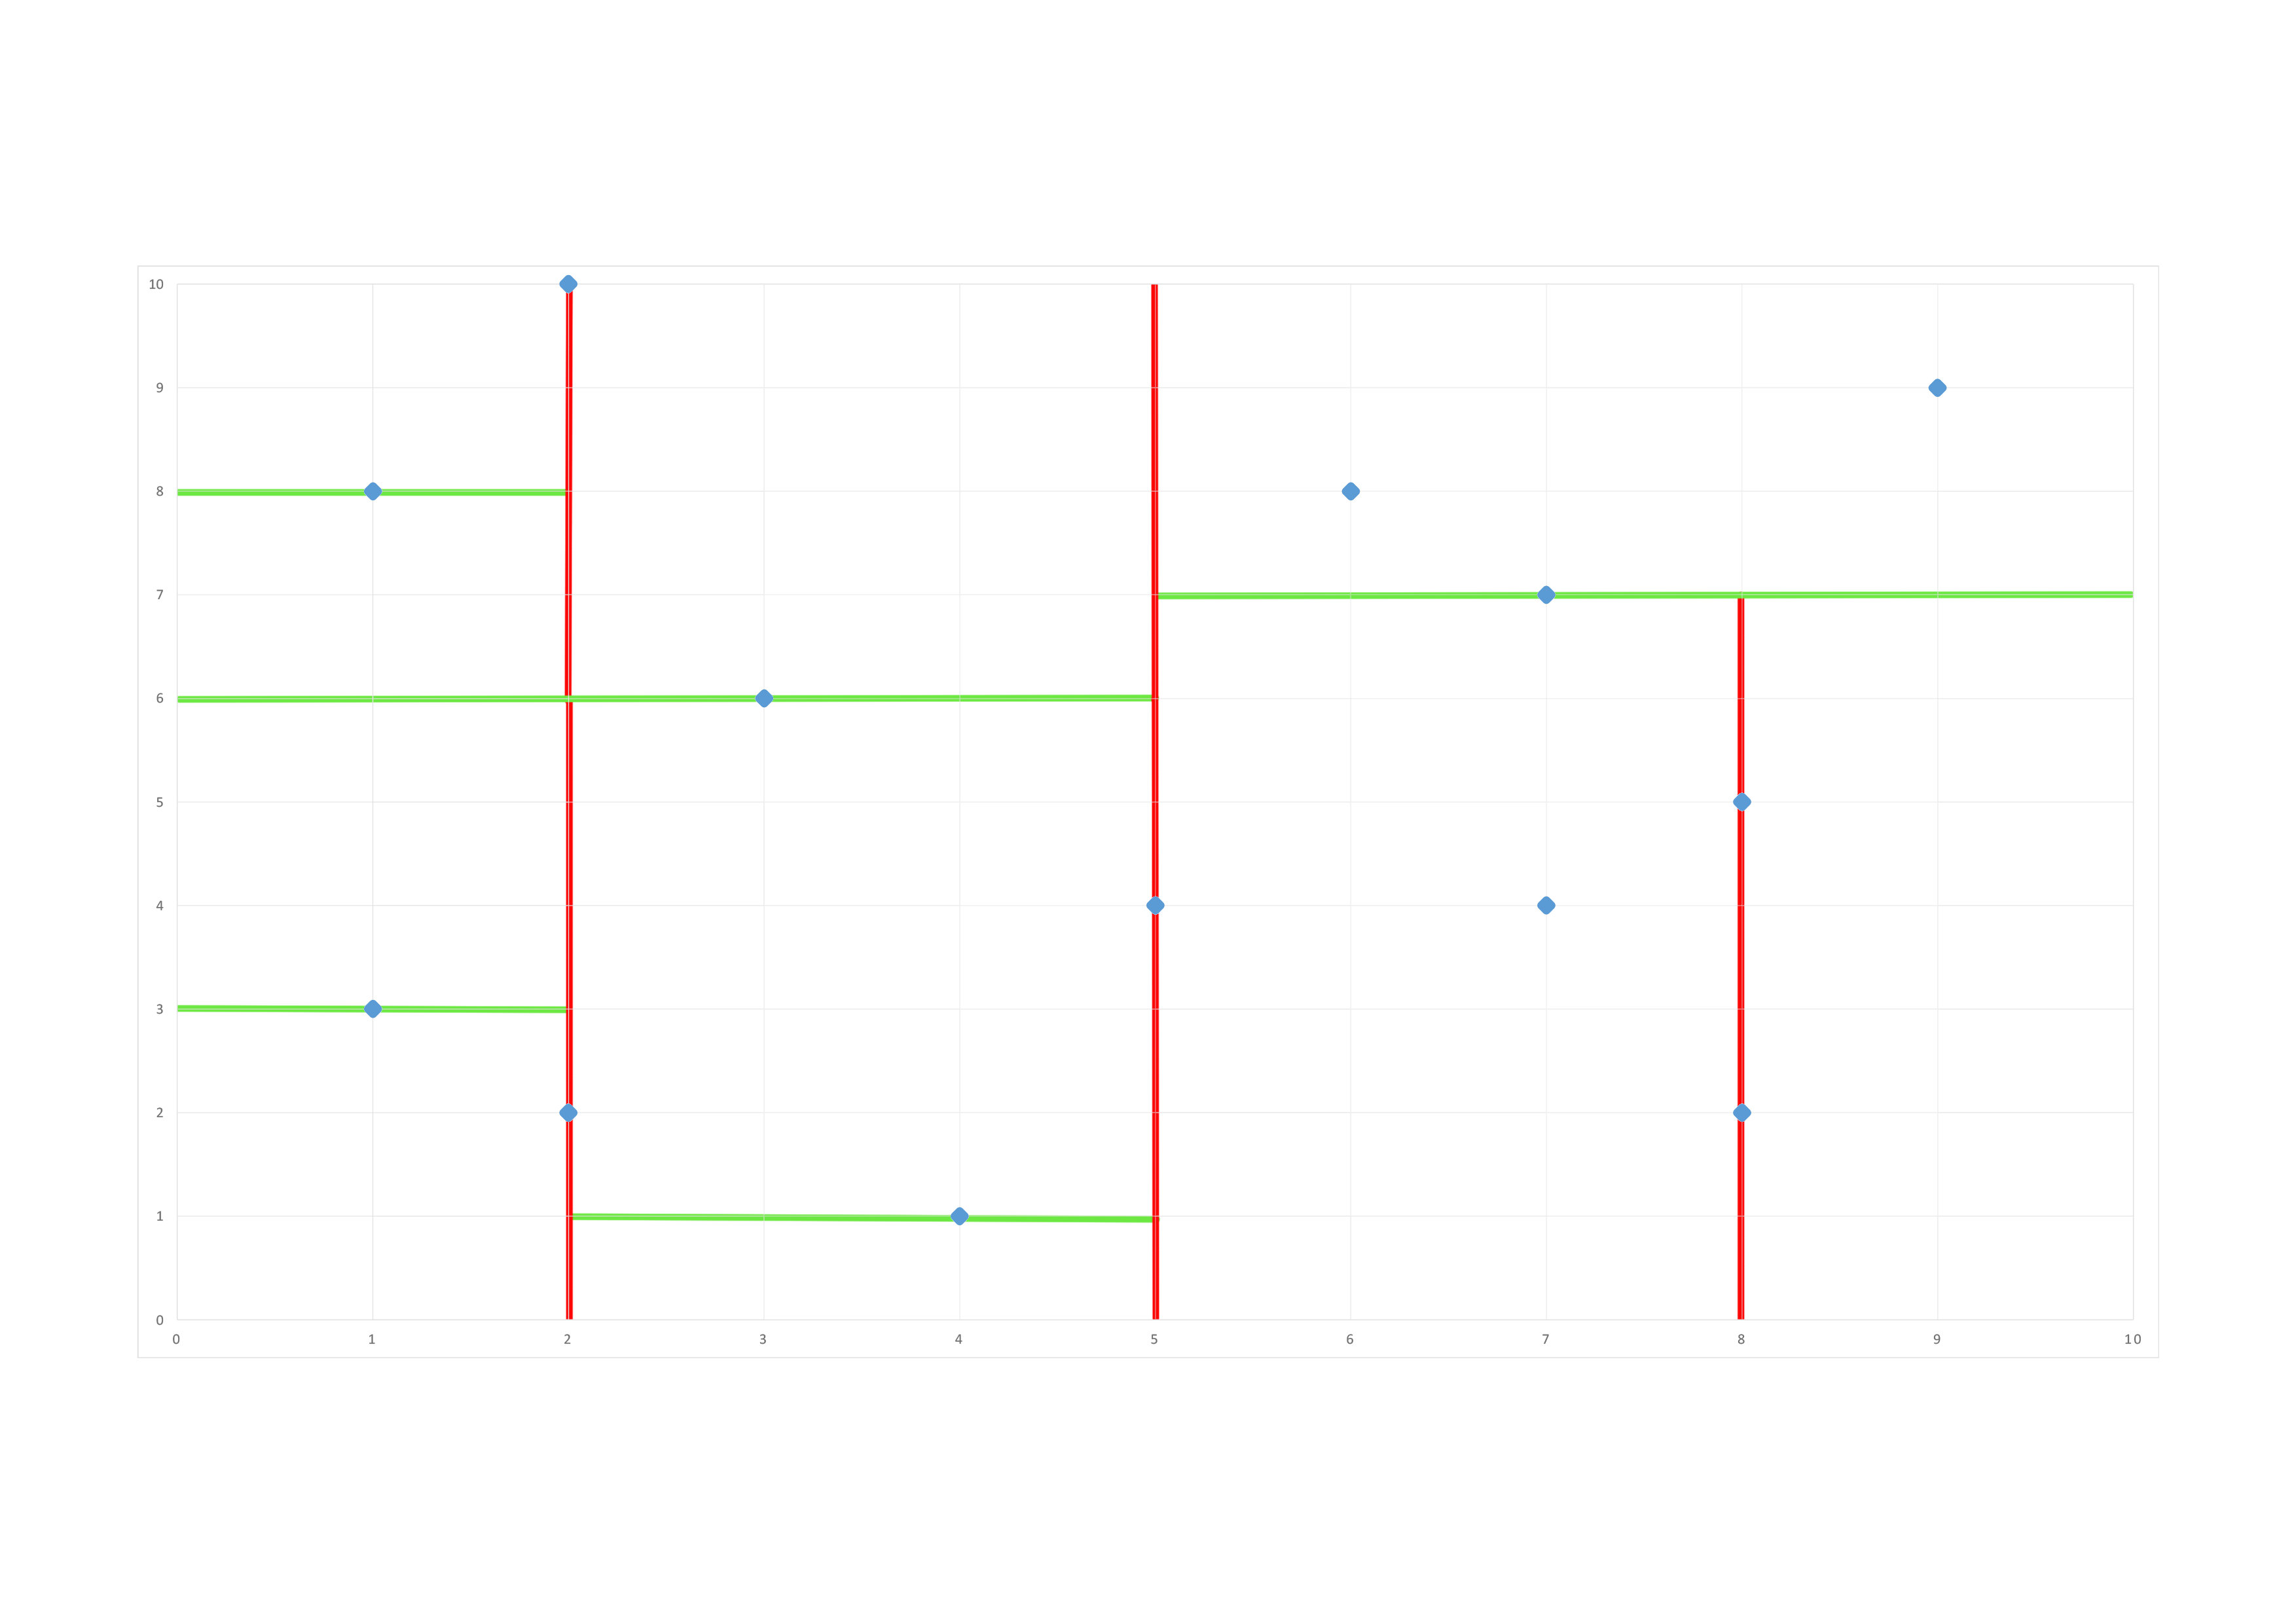
\includegraphics[width=.7\textwidth]{figures/split9.png}}
    \only<10>{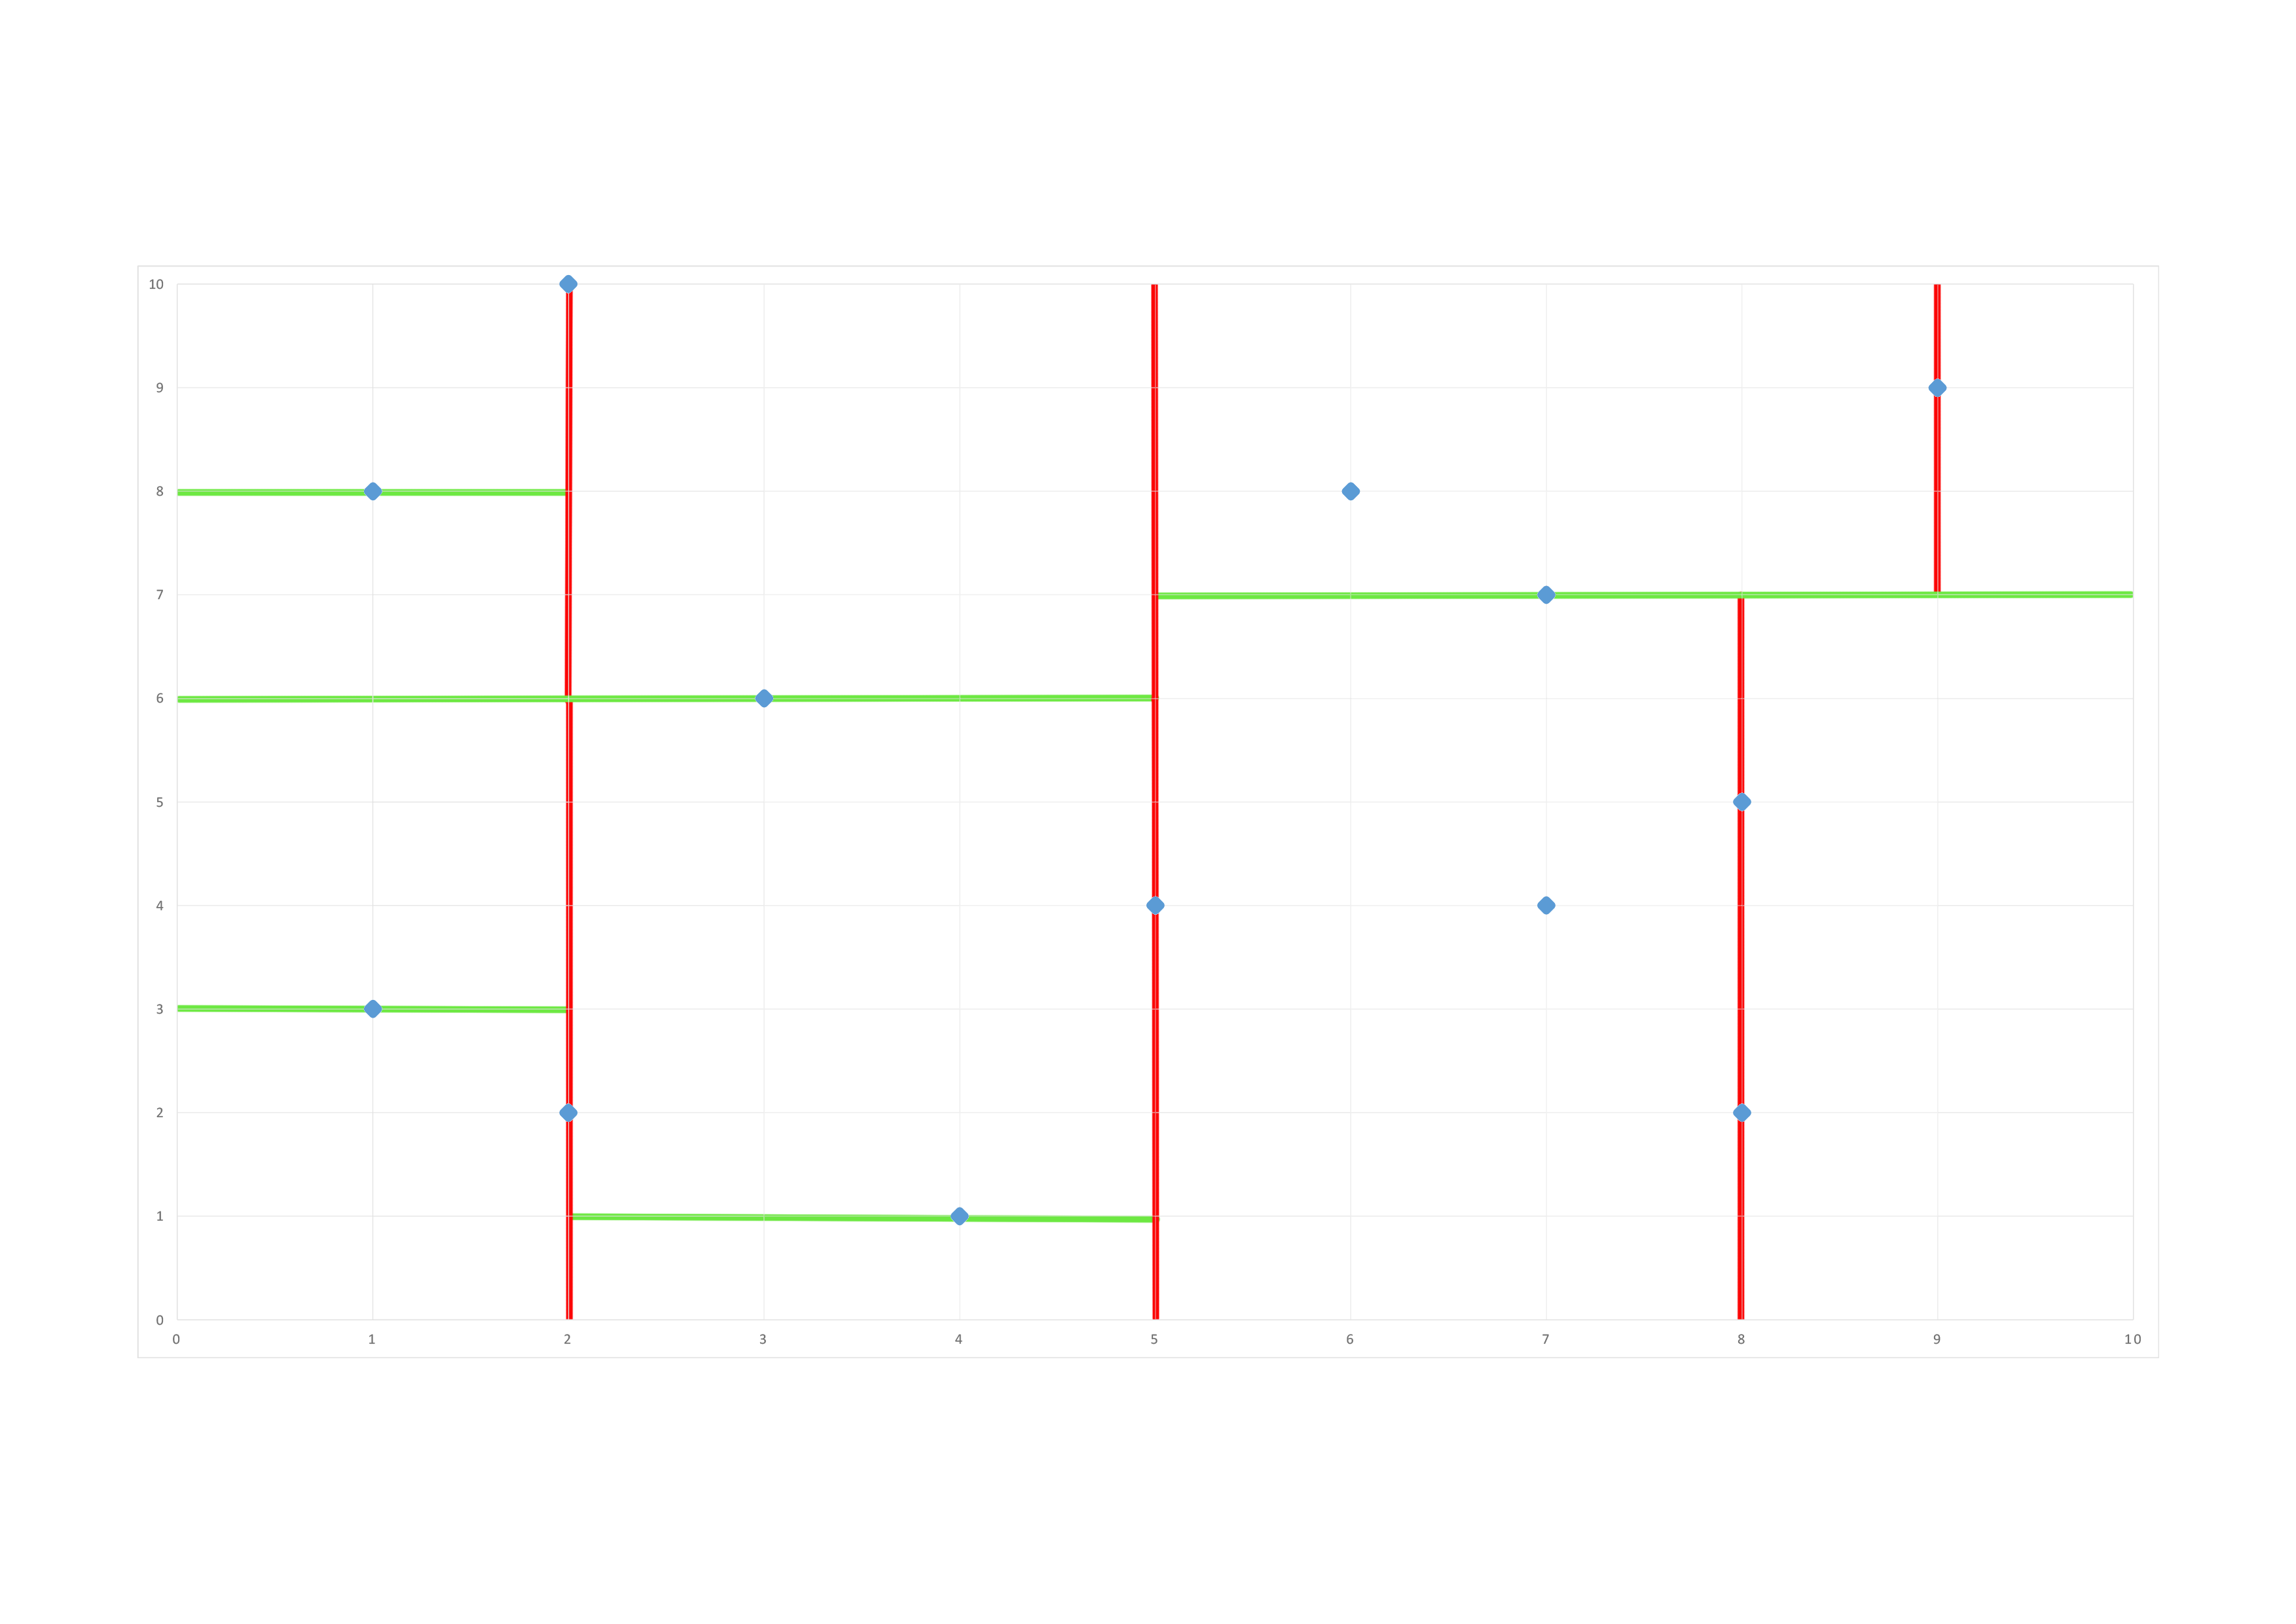
\includegraphics[width=.7\textwidth]{figures/split10.png}}
    \only<11>{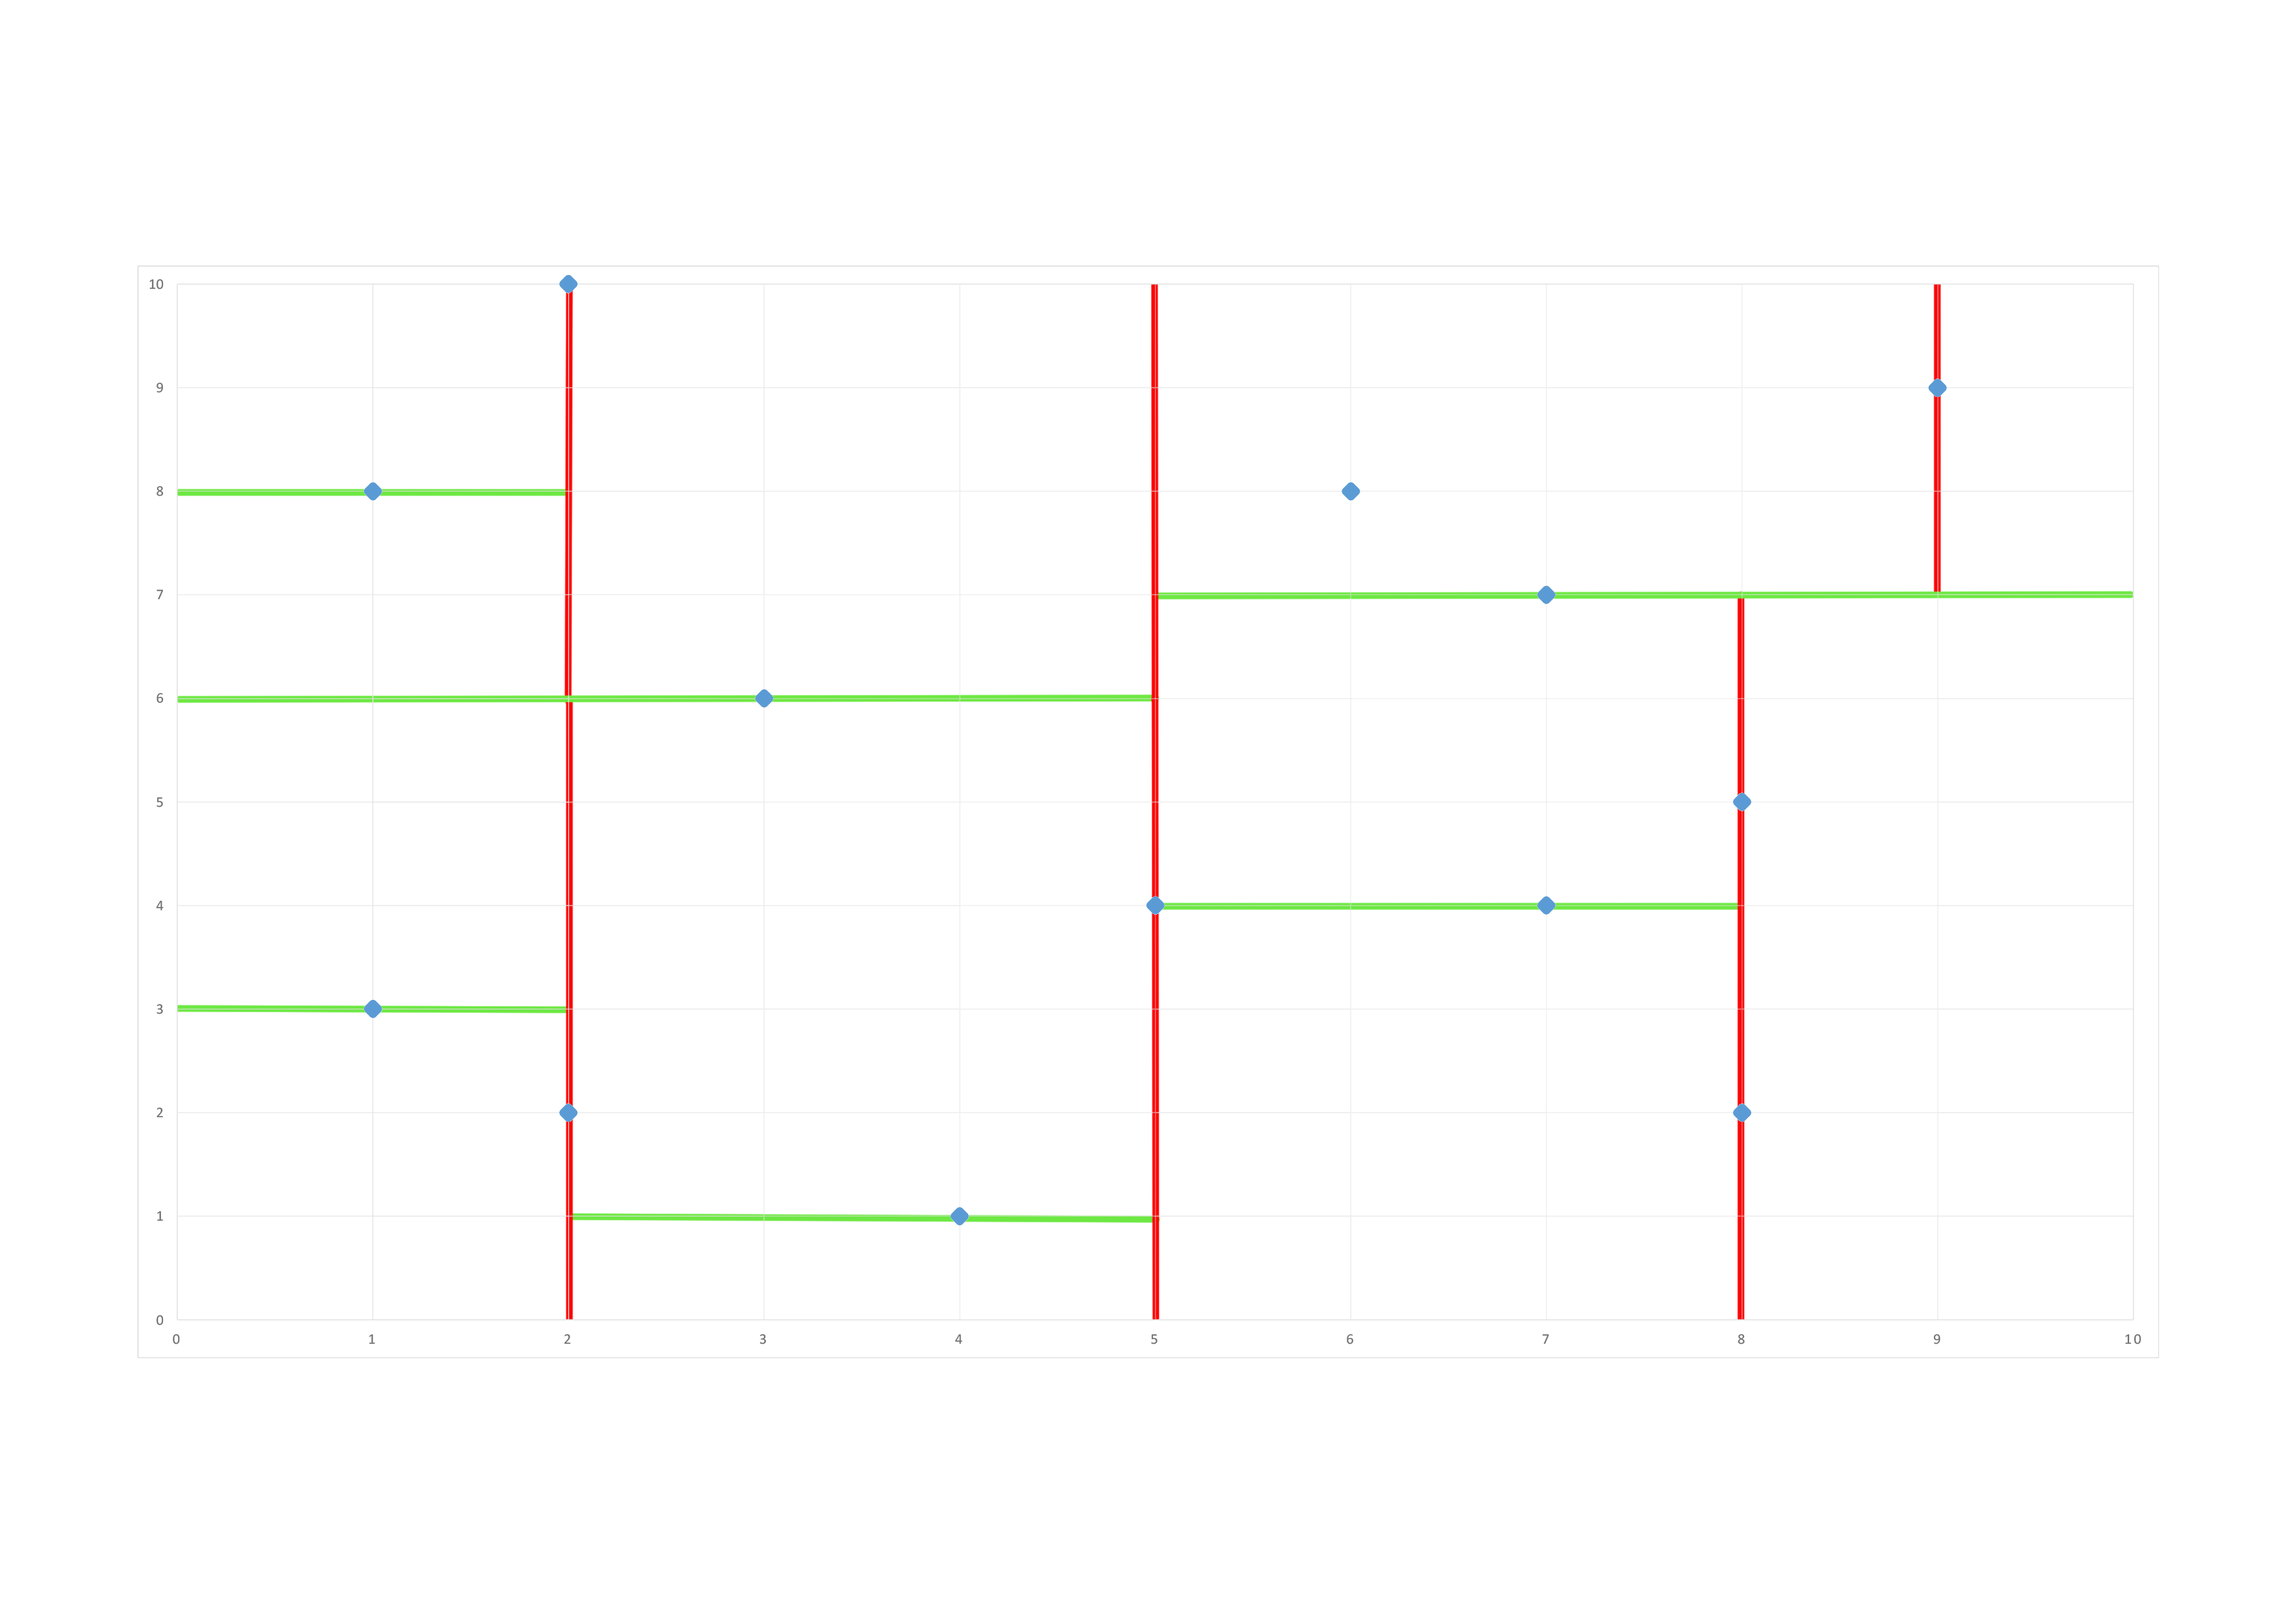
\includegraphics[width=.7\textwidth]{figures/split11.png}}
    \only<12>{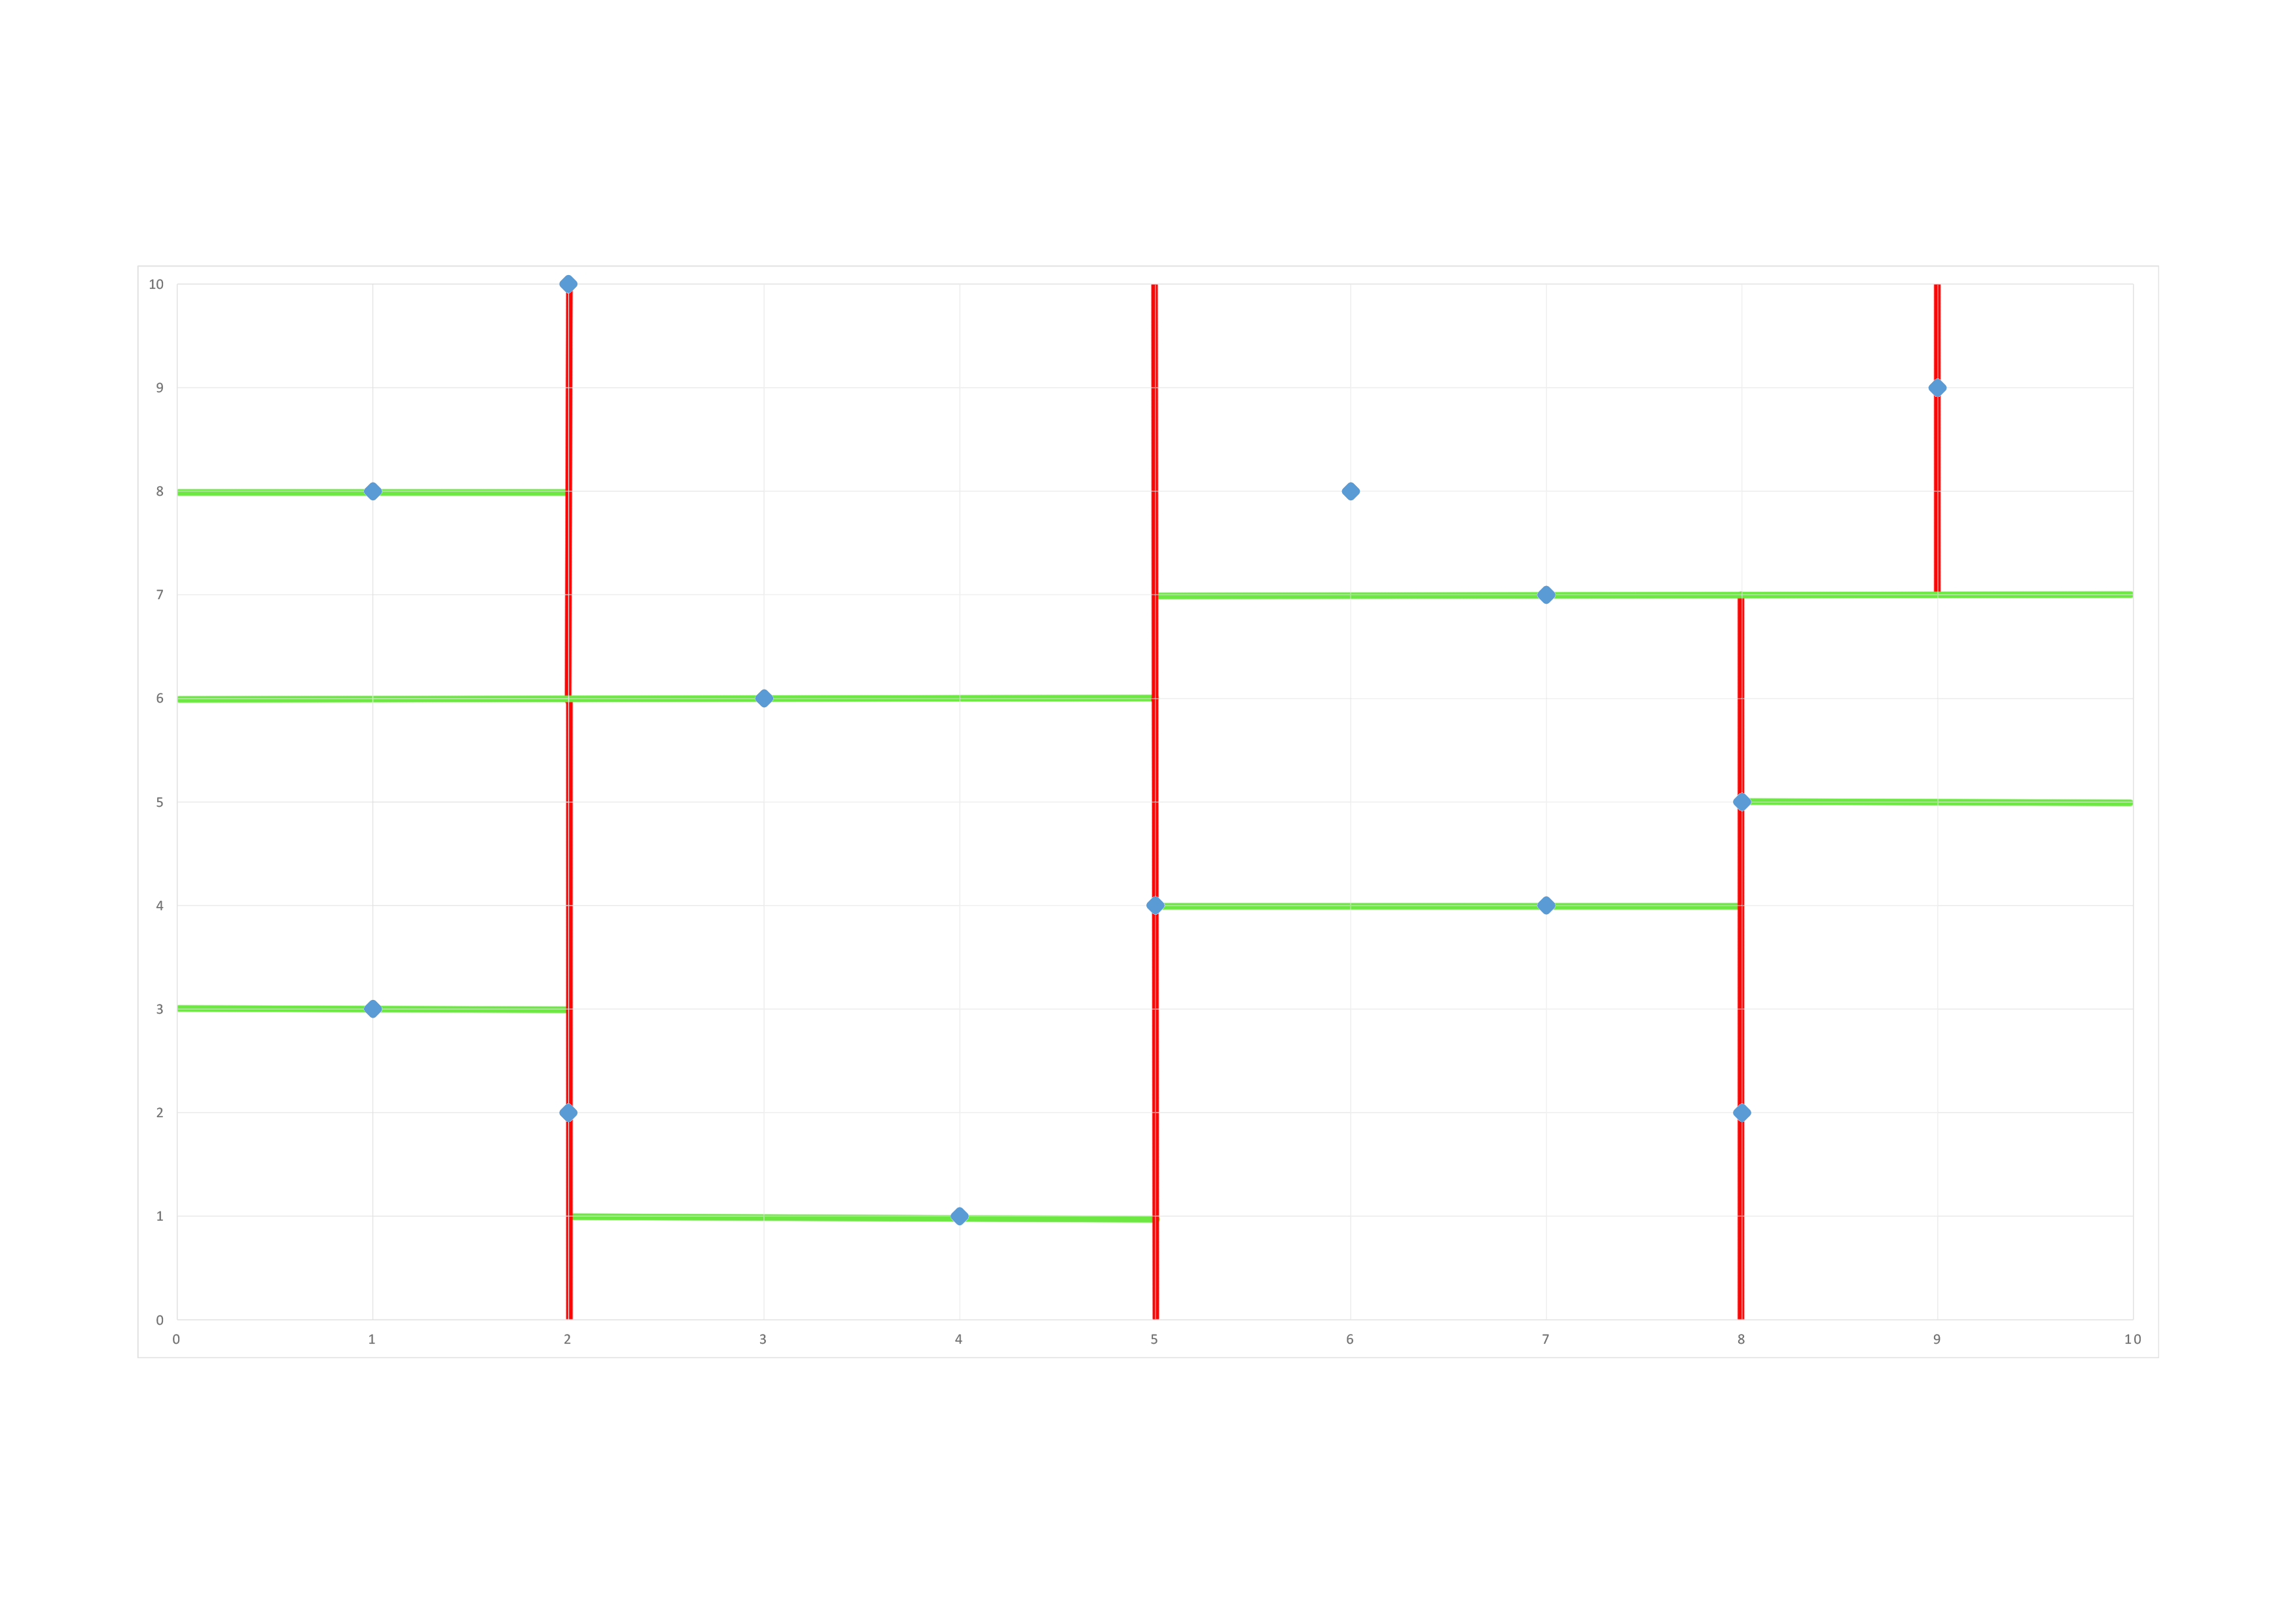
\includegraphics[width=.7\textwidth]{figures/split12.png}}
    \only<13>{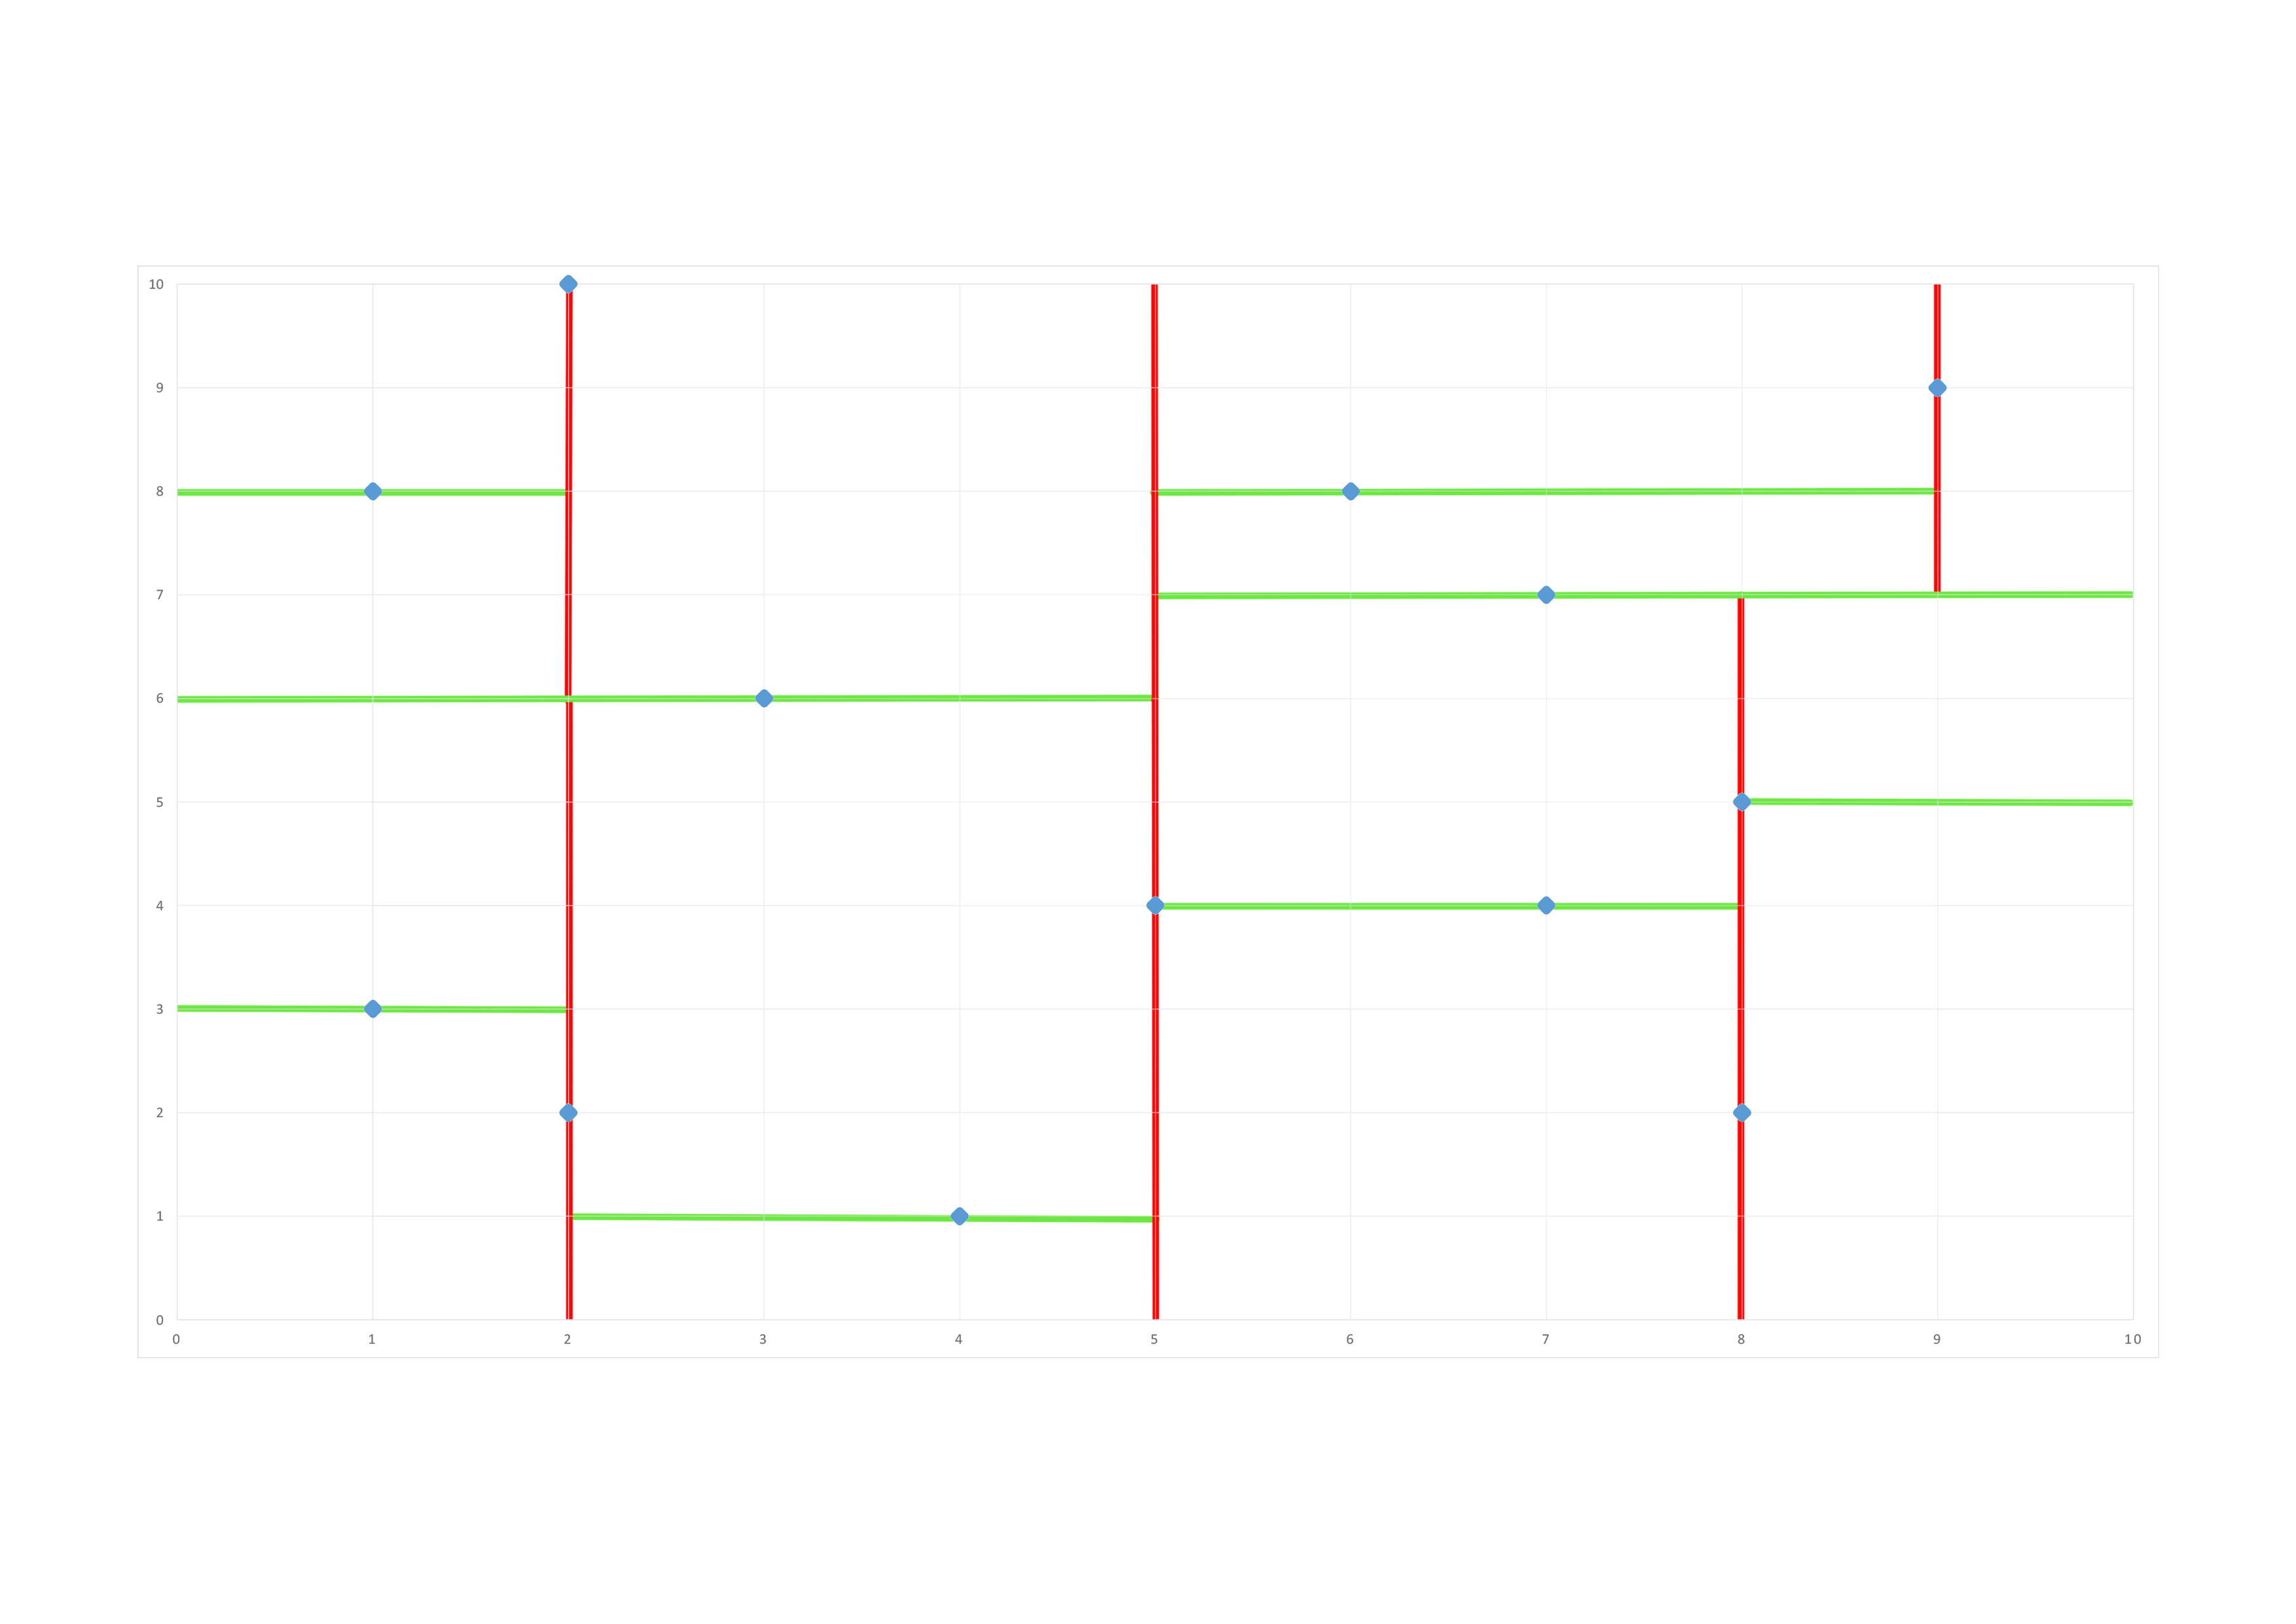
\includegraphics[width=.7\textwidth]{figures/splitFin.png}}
\end{frame}
%
\begin{frame}{how do we find the k nearest neighbours?}
  \begin{figure}
  	\centering
  	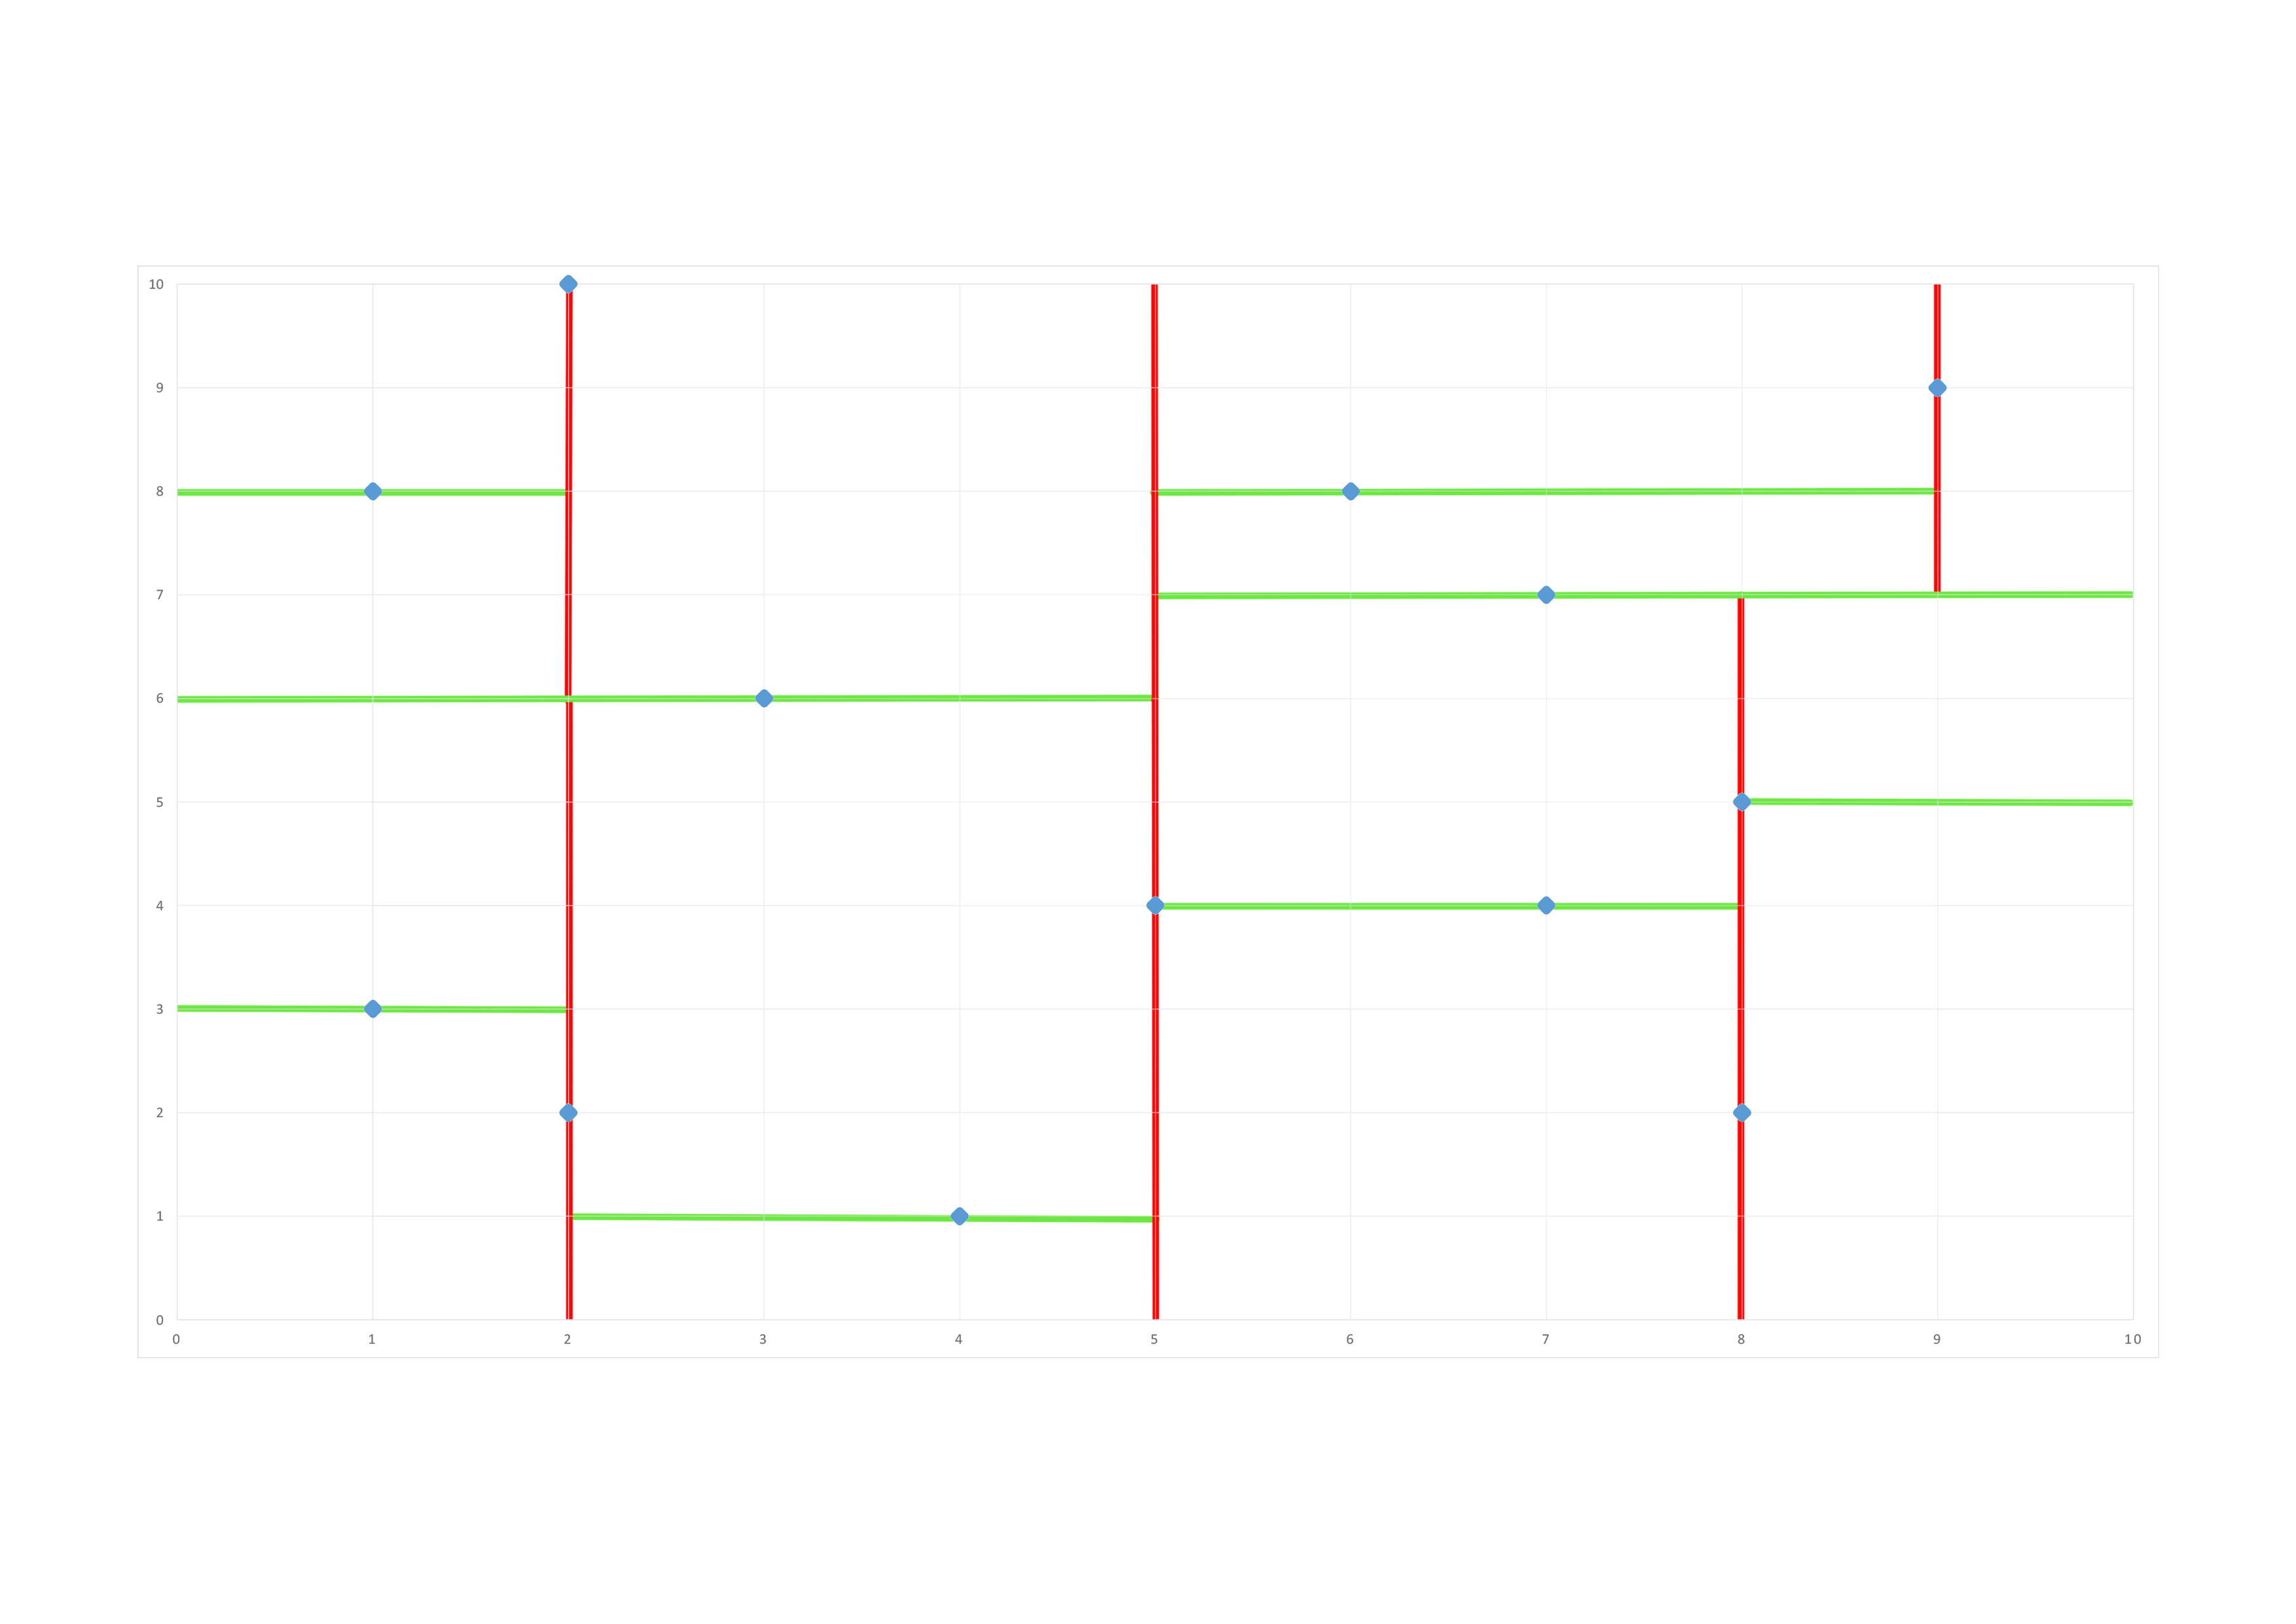
\includegraphics[width=.45\textwidth]{figures/splitFin.png}
  	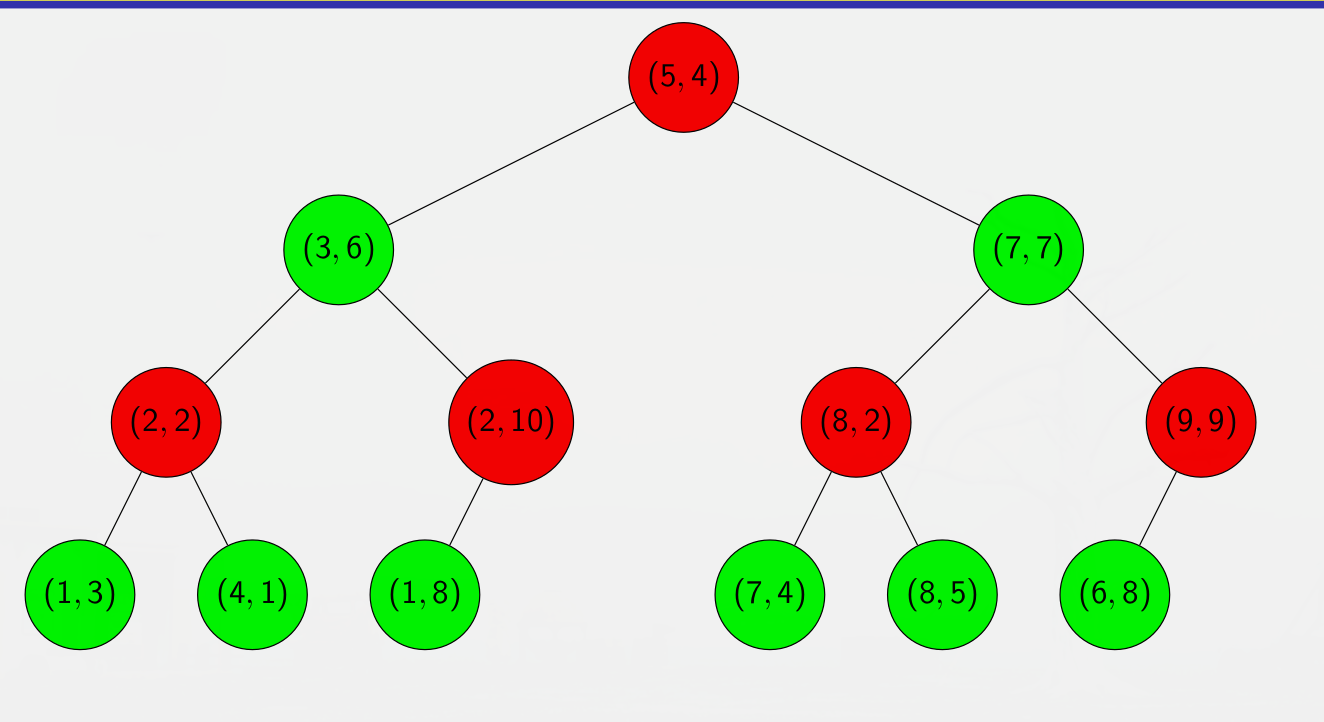
\includegraphics[width=.45\textwidth]{figures/tree.png}
  \end{figure}
\end{frame}

\begin{frame}{What is the time complexity?}
  For the tree creation (best case):
  \begin{align*}
    T(n) &= nlog(n)+2T\left(\frac{n}{2}\right)\\
         &= nlog(n)+2\left(\frac{n}{2}log\left(\frac{n}{2}\right)+2T\left(\frac{n}{4}\right)\right)\\
         &= nlog(n)+nlog\left(\frac{n}{2}\right)+4T\left(\frac{n}{4}\right)\\
         &= nlog(n)+nlog\left(\frac{n}{2}\right)+nlog\left(\frac{n}{4}\right)+\cdots+nlog\left(\frac{n}{2^{log(n)}}\right)\\
         &= n\sum^{log(n)}_{i=0}log\left(\frac{n}{2^i}\right)\\
         &= o\left(n\sum^{log(n)}_{i=0}log(n)\right)\\
         &= o(nlog^2(n))
  \end{align*}
\end{frame}

\begin{frame}{What is the time complexity?}
  For the tree creation (worst case):
  \begin{align*}
    T(n) &= n^2 +2T\left(\frac{n}{2}\right)\\
         &= n^2 +2\left(\left(\frac{n}{2}\right)^2+2T\left(\frac{n}{4}\right)\right)\\
         &= \sum^{log(n)}_{i=0}\frac{n^2}{2^i}\\
         &= n^3(2-2^{-log(n)})\\
         &= o(n^3)
  \end{align*}
\end{frame}
%
\begin{frame}{what is the time complexity}
  time complexity of our full program:
  \smallskip
  \begin{itemize}
  \item For the nearest neighbour search:
  \begin{itemize}
    \item best: $T(n)=o(log(n)d)$
    \item worst: $T(n)=o(nd)$ \emph{$\equiv$ depth-first traversal}
  \end{itemize}
  \item For k-nearest neighbours of $p$ points:
  \begin{itemize}
    \item best:
    \begin{itemize}
      \item if $pd>nlog(n) \Rightarrow T(n) = o(pdlog(n))$
      \item otherwise $T(n) = o(nlog^2(n))$
    \end{itemize}
    \item worst:
    \begin{itemize}
      \item if $pd>n^2 \Rightarrow T(n)=o(pdn)$ (very unlikely)
      \item otherwise $T(n)=o(n^3)$
    \end{itemize}
  \end{itemize}
\end{itemize}
\smallskip
Most of the complexity is due to tree creation.\\\smallskip
$k$-fold cross validation does not increase complexity unless the number of folds is very high.
\end{frame}
%
\begin{frame}{How does our program perform?}
  \begin{figure}
    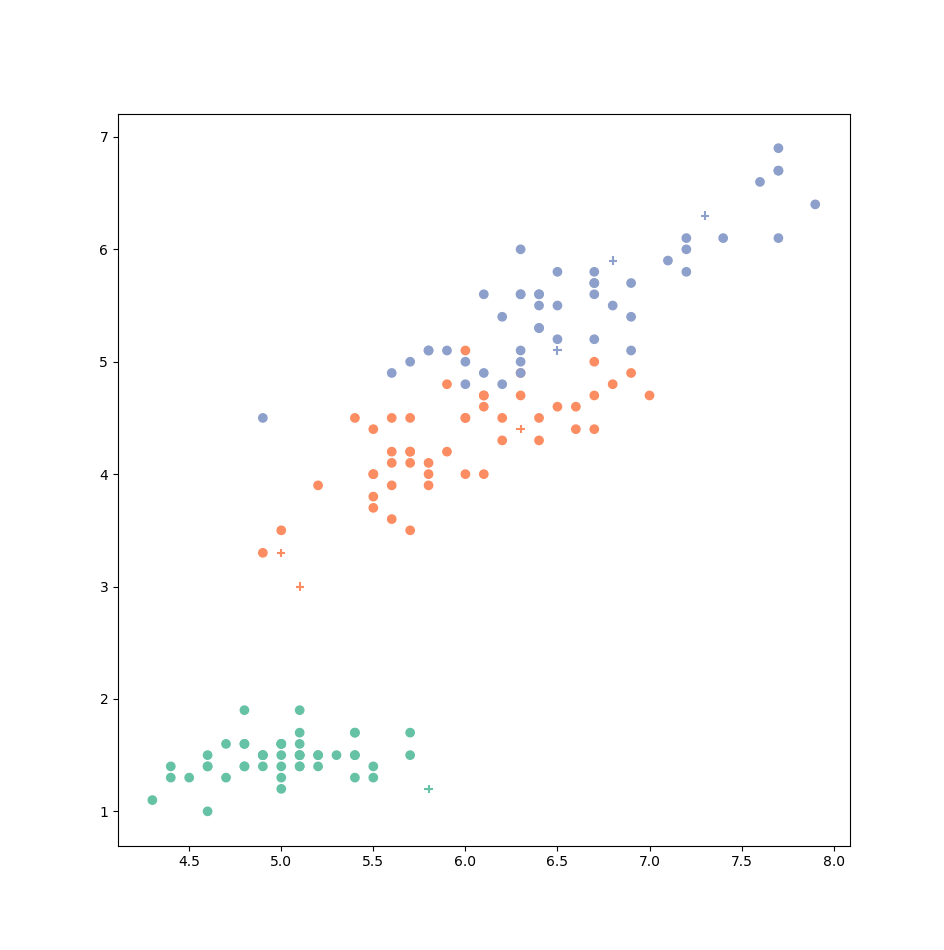
\includegraphics[width=.7\textwidth]{figures/iris3.png}
    \caption{classification of points in the iris dataset}
  \end{figure}
\end{frame}

\begin{frame}{How does our program perform?}
  \begin{figure}
    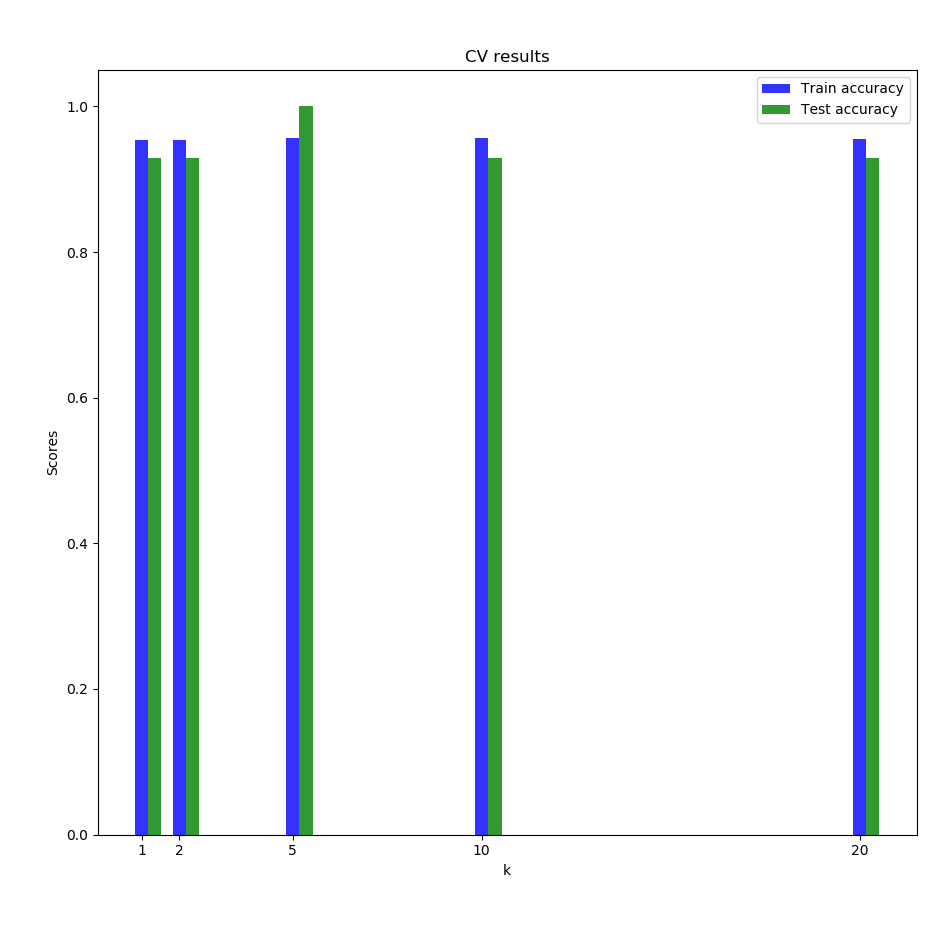
\includegraphics[width=.7\textwidth]{figures/iris3Cv2.png}
    \caption{Cross validation results on iris}
  \end{figure}
\end{frame}

\begin{frame}{does it work for bigger spaces?}
\begin{figure}
  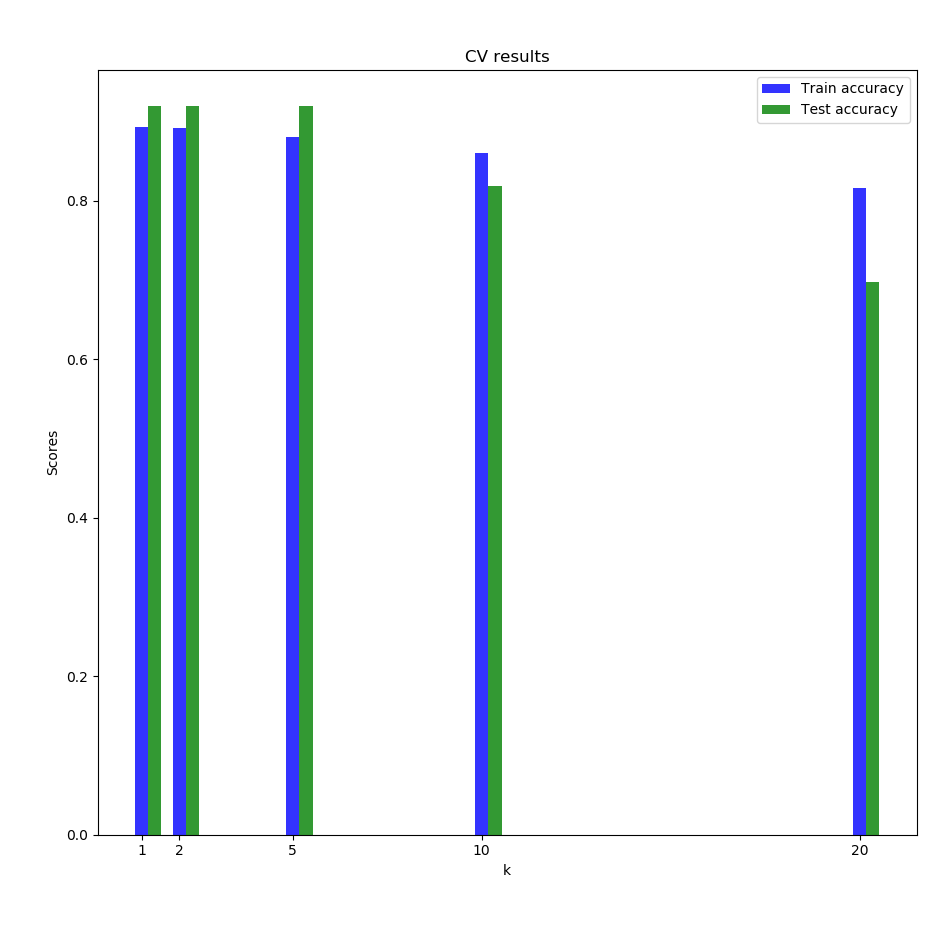
\includegraphics[width=.55\textwidth]{figures/leafCv.png}
  \caption{CV results on leaf dataset \emph{(d=192, 99 classes, n=990)}}
\end{figure}
\end{frame}

\section{Improvements, and future works}

\begin{frame}
\begin{itemize}
  \item Implement approximative in CV then apply exact Knn with optimal k
  \item be able to handle categorical data
  \item implement faster median selection algorithm (for faster tree creation)
\end{itemize}
\end{frame}

\end{document}
